\documentclass[a4paper, italian, openany]{book}
\usepackage[italian]{babel}
\usepackage[latin1]{inputenc}
\usepackage{amsmath}
\usepackage[pdftex]{graphicx}
\usepackage{siunitx}
\usepackage{enumerate}
\usepackage{float}
\usepackage{fancyhdr}
\usepackage{listings}
\usepackage[a4paper]{geometry}
\newcommand{\HRule}{\rule{\linewidth}{0.5mm}}

\lstdefinestyle{customc}{
  belowcaptionskip=1\baselineskip,
  breaklines=true,
  frame=L,
  xleftmargin=\parindent,
  language=C,
  showstringspaces=false,
  basicstyle=\footnotesize\ttfamily,
  keywordstyle=\bfseries\color{green!40!black},
  commentstyle=\itshape\color{purple!40!black},
  identifierstyle=\color{blue},
  stringstyle=\color{orange},
}

\lstdefinestyle{customasm}{
  belowcaptionskip=1\baselineskip,
  frame=L,
  xleftmargin=\parindent,
  language=[x86masm]Assembler,
  basicstyle=\footnotesize\ttfamily,
  commentstyle=\itshape\color{purple!40!black},
}

\lstset{escapechar=@,style=customc}

\begin{document}
\pagestyle{fancy}
\pagestyle{plain}

\begin{titlepage}
\begin{center}


\includegraphics[width=0.9\textwidth]{sissa.jpg}~\\[1cm]

\HRule \\[0.4cm]
{ \large \bfseries Numerical Methods II - Statistical Mechanics and Molecular Dynamics \\[0.4cm] }

\HRule \\[1.5cm]

\noindent
\begin{minipage}[t]{0.4\textwidth}
\begin{flushleft} \large
\emph{Professori:}\\
G. \textsc{Bussi}\\
C. \textsc{Micheletti}
\end{flushleft}
\end{minipage}
\begin{minipage}[t]{0.4\textwidth}
\begin{flushright} \large
\emph{Autore:} \\
Iacopo \textsc{Poli}\\
\end{flushright}
\end{minipage}

\vfill

{\small \today}

\end{center}
\end{titlepage}

\tableofcontents

\chapter{Statistical Mechanics}

For reference you can look to ch. 6-7 of \textit{Statistical Mechanics}, Kerson, Huang, MIT.

\section{Postulate of Classical Statistical Mechanics}

Statistical mechanics concerns equilibrium properties of systems, it doesn't study how the system approaches the equilibrium nor if it can reach it, only what the situation at equilibrium is for a given system.\newline
Statistical mechanics studies systems at thermodynamic equilibrium. In particular we assume to be in \textit{thermodynamic limit}: N, V are large enough that it makes sense to introduce $n = \frac{N}{V}$ and $N \rightarrow \infty, V \rightarrow \infty$ but $n$ is fixed and constant (volume and number of particles grow in proportion).\newline
In the study of gas of N particles, we introduce 3N $q_I$ coordinates and 3N $p_i$ coordinates. Weak interactions are assumed, in order to let the system reach equilibrium, but apart from this, the motion is governed by Hamilton equations of motion.

$$\dot{q_i} = \frac{\partial H}{\partial p_i}$$
$$\dot{p_i} = - \frac{\partial H}{\partial q_i}$$

\begin{figure}[H]
\centering
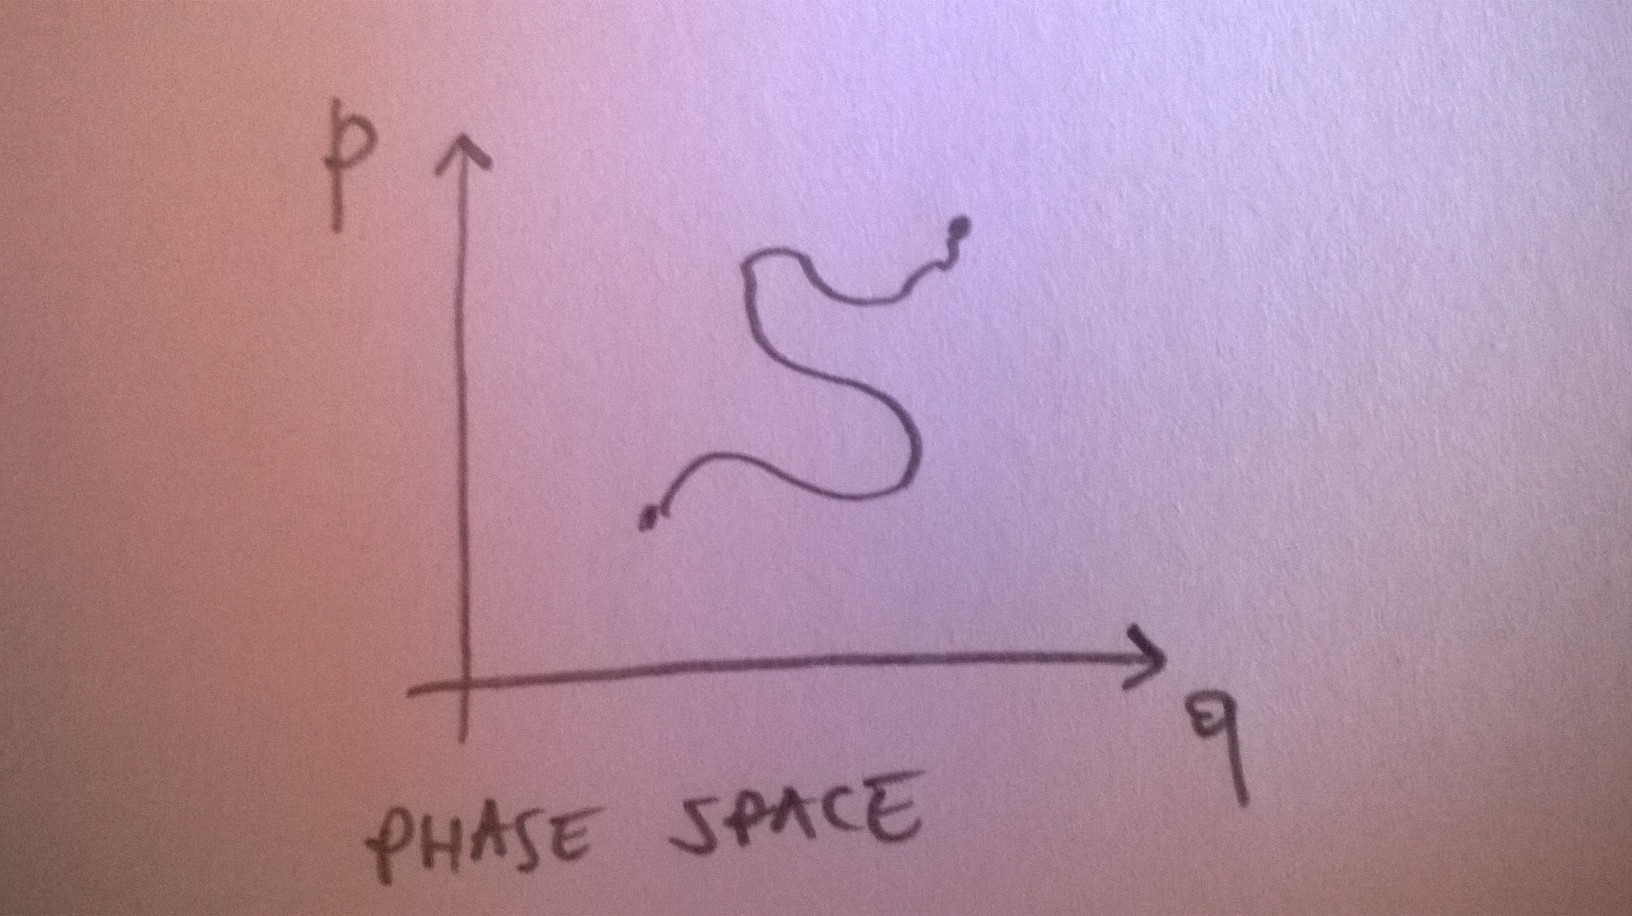
\includegraphics[width=100mm]{figure1.jpg}
\end{figure}

In the phase space, trajectories that intersect themselves are not allowed, since at the intersection I wouldn't know where to proceed and this would imply a non-deterministic behavior. Given this rule, I can have two kinds of trajectories:
\begin{itemize}
\item closed curves: they conserve the energy, but don't equilibrate, for example, harmonic oscillators.
\item curves that fill out the space compatible with constraints on the system without self-intersecting or closing.
\end{itemize}


\begin{figure}[H]
\centering
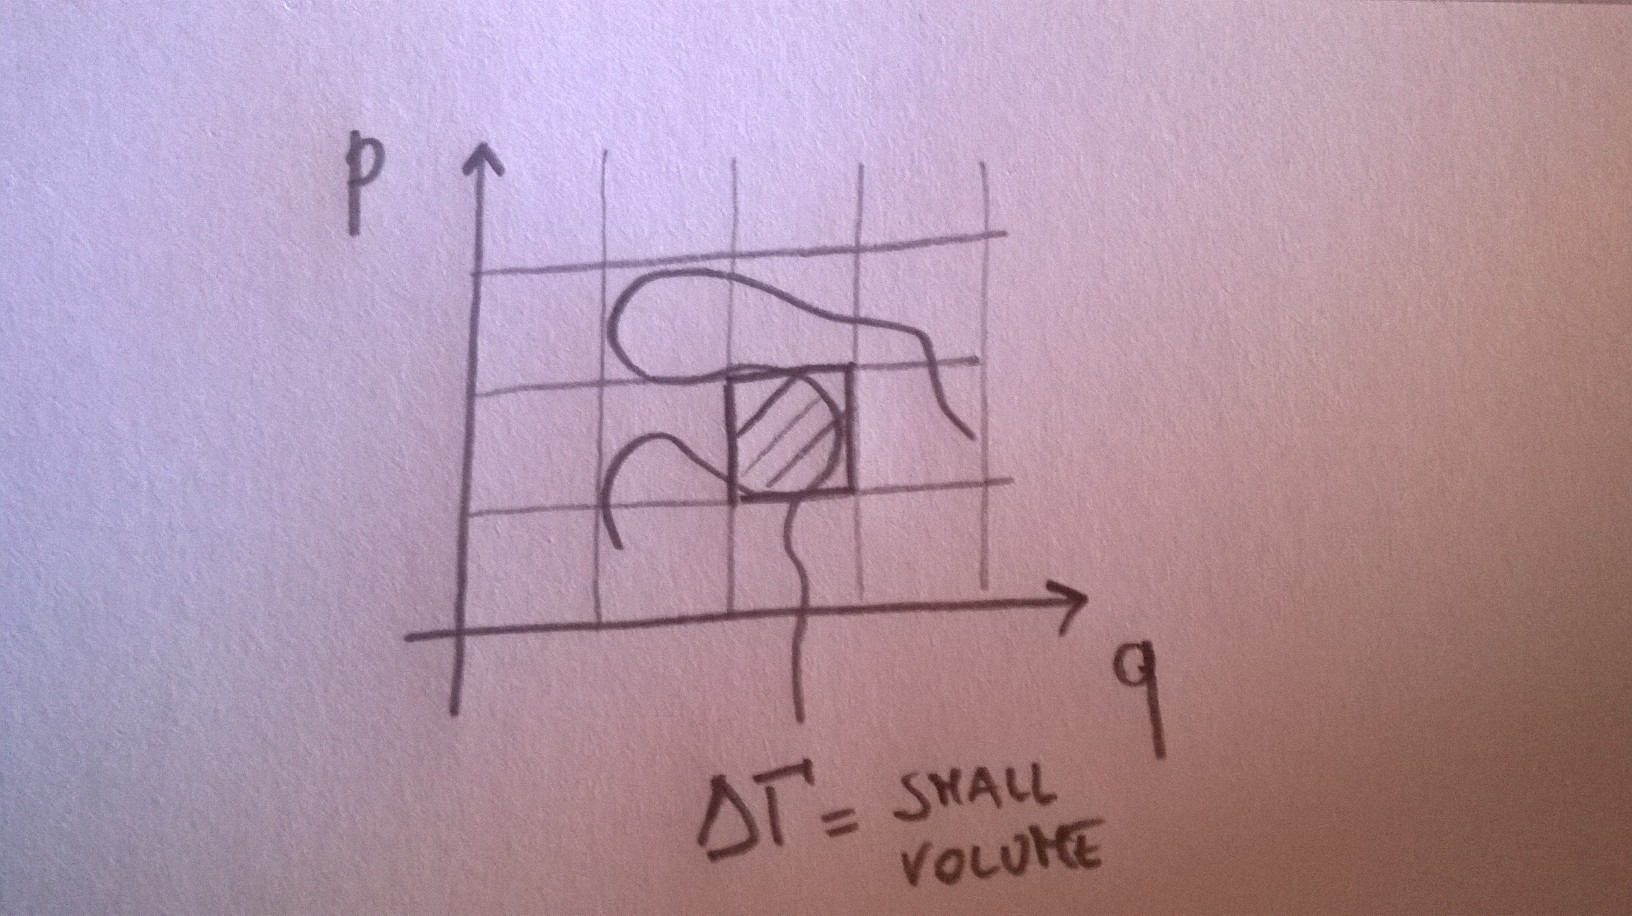
\includegraphics[width=70mm]{figure2.jpg}
\end{figure}

If we divide the phase space in small volumes $\Delta \Gamma$, we can build an histogram adding +1 every time the system visits a particular spot of the grid. At the end we will have an histogram of how many times that state has been visited by the system. The dimension of the volume gives the precision of momenta and coordinates: it is the level of fine graining.\newline
We want to know how much time the system spends in every bin:

$$\lim_{T \to \infty} \frac{\Delta t_i(\Gamma_i)}{T} = \rho(\overrightarrow{q_i}, \overrightarrow{p_i}) \cdot \Delta \Gamma$$ 

if the system is in equilibrium, where $\rho(\overrightarrow{q_i}, \overrightarrow{p_i})$ is a probability density.\newline
Let's take $f(\overrightarrow{q}, \overrightarrow{p})$ as a generic observable:

$$<f> = \lim_{T \to \infty} \frac{1}{T} \int_0^T dt f(\overrightarrow{q}(t), \overrightarrow{p}(t)) = \lim_{T \to \infty} \frac{1}{T}\sum_i \Delta t(q_i, p_i) \cdot f(q_i, p_i)$$

since $\lim_{T \to \infty} \frac{1}{T} \Delta t(q_i, p_i) = \rho_i$:

$$<f> = \sum_i \lim_{T \to \infty} \frac{\Delta t_i}{T} \cdot f(\overrightarrow{q_i}, \overrightarrow{p_i}) = \sum_i \rho(\overrightarrow{q_i}, \overrightarrow{p_i}) \cdot \Delta \Gamma \cdot f(\overrightarrow{q_i}, \overrightarrow{p_i}) = \int d\Gamma  f(\overrightarrow{q}, \overrightarrow{p})\cdot \rho(\overrightarrow{q}, \overrightarrow{p}))$$

The expected value of an observable can be computed as time average of a very long trajectory, or value of observable in any point of the phase space per a weight of time spent in that point.

\textbf{Ensemble}: a collection of mental copies of the system picked with an appropriate probability density function $\rho(\overrightarrow{q}, \overrightarrow{p})$

\paragraph{Liouville's Theorem}

\begin{figure}[H]
\centering
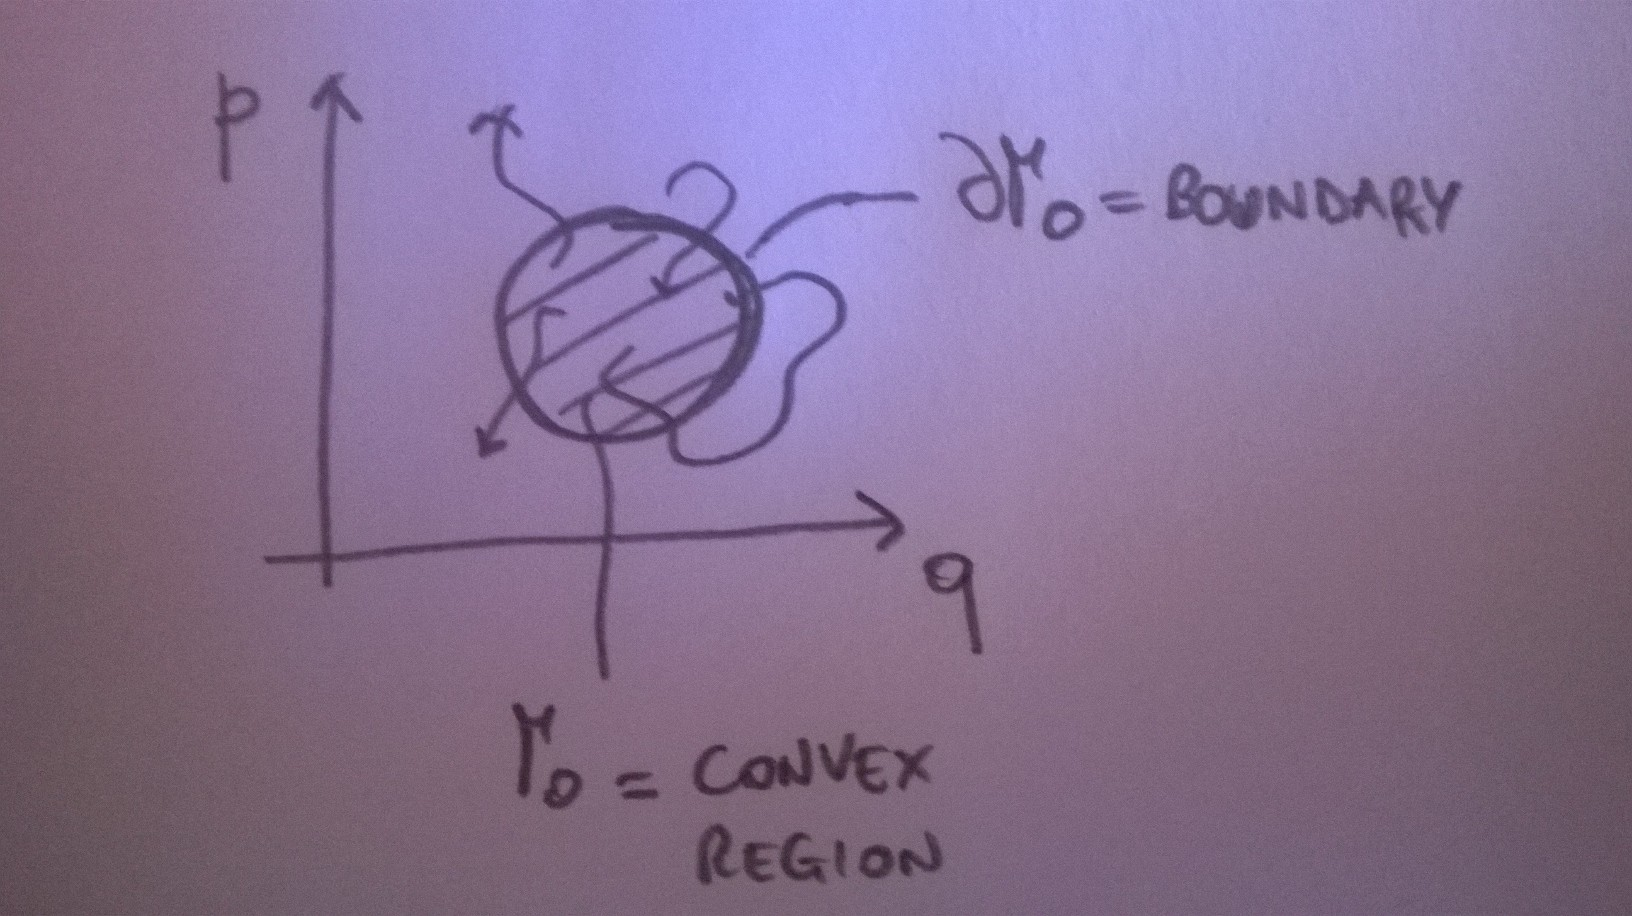
\includegraphics[width=70mm]{figure3.jpg}
\end{figure}

Let's choose a convex region $\Gamma_0$ of the phase space, whose boundary is $\partial \Gamma_0$. We can write:

$$-\frac{\partial}{\partial t} \int_{\Gamma_0} d\Gamma \rho = \int_{\partial \Gamma_0} dS \overrightarrow{n} \cdot (\rho \cdot \overrightarrow{v})$$

and using Gauss' Theorem:

$$\int_{\partial \Gamma_0} dS \overrightarrow{n} \cdot (\rho \cdot \overrightarrow{v}) =  \int_{\Gamma_0} d\Gamma \overrightarrow{\nabla} \cdot (\rho \cdot \overrightarrow{v})$$

since the choice of $\Gamma_0$ is arbitrary, this implies:

$$-\frac{\partial \rho}{\partial t} = \overrightarrow{\nabla} \cdot (\rho \cdot \overrightarrow{v})$$

exploit divergence:

$$-\frac{\partial \rho}{\partial t} = \sum_{i=1}^{3N} \left [ \frac{\partial \rho}{\partial q_i}\dot{q_i} + \frac{\partial \rho}{\partial p_i} \dot{p_i} \right ] + \rho \sum_{i=1}^{3N} \left [ \frac{\partial}{\partial q_i}\dot{q_i} + \frac{\partial}{\partial p_i} \dot{p_i} \right ]$$

since $\left [ \frac{\partial}{\partial q_i}\dot{q_i} + \frac{\partial}{\partial p_i} \dot{p_i} \right ] = \left [ \frac{\partial^2 H}{\partial q_i \partial p_i} - \frac{\partial^2 H}{\partial p_i \partial q_i} \right ] = 0$

$$\sum_{i=1}^{3N} \left [ \frac{\partial \rho}{\partial q_i} \frac{\partial q_i}{\partial t} + \frac{\partial \rho}{\partial p_i} \frac{\partial p_i}{\partial t} \right ] + \frac{\partial \rho}{\partial t} = 0$$

and the left hand side is the definition of total derivative of $\rho$ in time:

$$\frac{d\rho}{dt} = 0$$

which is the Liouville's theorem: \textit{total derivative of $\rho$ with respect to time is zero, which means probability density $\rho$ is constant with time}.

\section{Microcanonical ensemble}

Let's consider a system with weak interactions, in which $\varepsilon < H < \varepsilon + \Delta \varepsilon$, so that a priori probability postulate is:

$$\rho(\overrightarrow{q}, \overrightarrow{p}) = \begin{cases}\mbox{const} \mbox{,   if   } H(\overrightarrow{q}, \overrightarrow{p}) \epsilon \left [ \varepsilon , \varepsilon + \Delta \varepsilon \right ] \\ 0 \mbox{,   otherwise}\end{cases}$$

We define entropy as:

$$S(E) = K_B ln(\Gamma_\Delta(E))$$

where $\Gamma_\Delta(E) = \iint \limits_{\varepsilon < H < \varepsilon + \Delta \varepsilon} d^{3N}q d^{3N}p \cdot 1$.\newline 
Since entropy is an extensive property,  $S_{1+2} = S_1 + S_2$ must hold.

\begin{figure}[H]
\centering
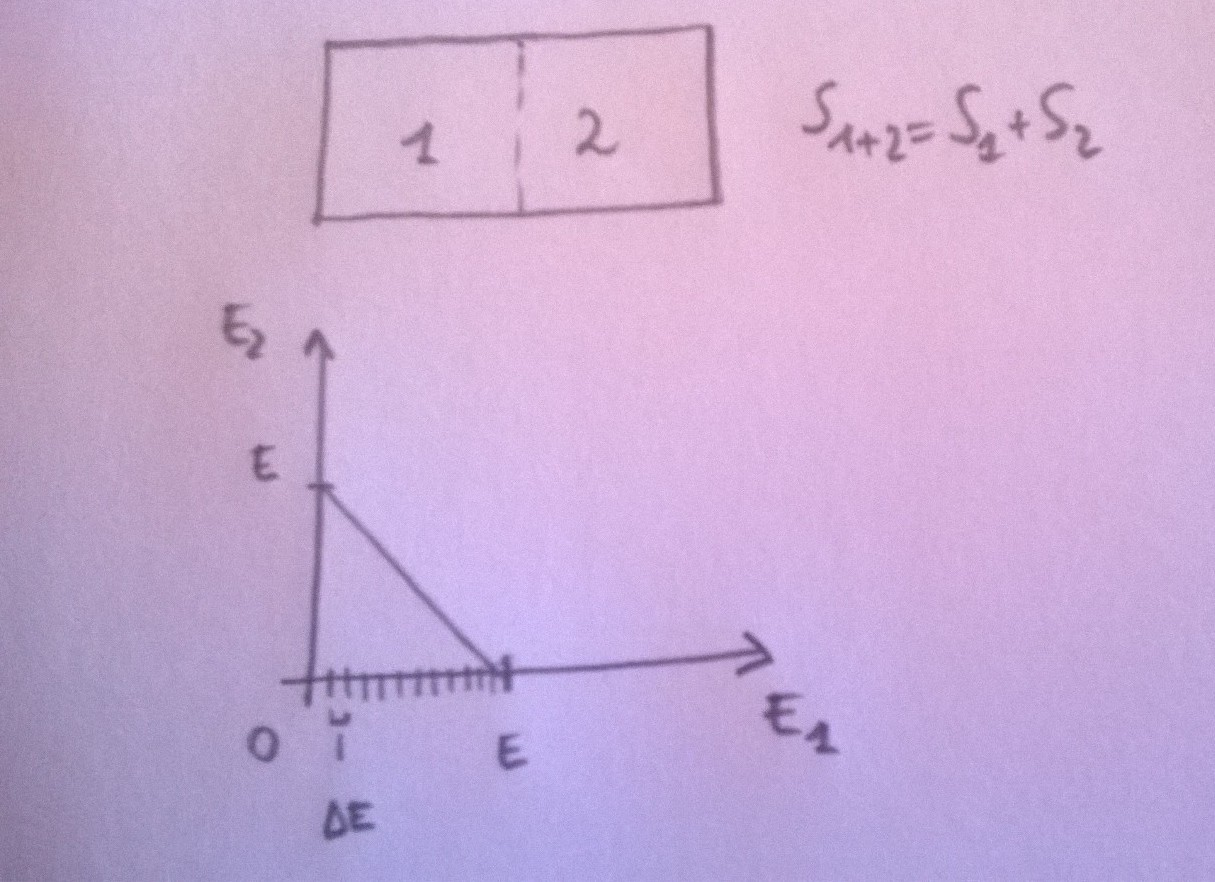
\includegraphics[width=100mm]{figure4.jpg}
\end{figure}

if I know $E_1$, then $E_2 = E- E_1$. Then:

$$S_1 = K_B ln(\Gamma_1(E_1))$$
$$S_2 = K_B ln(\Gamma_2(E_2))$$

$$\Gamma_{1+2} = \sum_{E_1=0}^{E} \Gamma_1(E_1) \cdot \Gamma_2(E-E_1)$$

by construction:

$$\Gamma_1(\bar{E_1})\cdot \Gamma_2(E- \bar{E_1}) \le \Gamma_{1+2} \le \Gamma_1(\bar{E_1})\cdot \Gamma_2(E-\bar{E_1}) \cdot \frac{E}{\Delta E}$$

\begin{figure}[H]
\centering
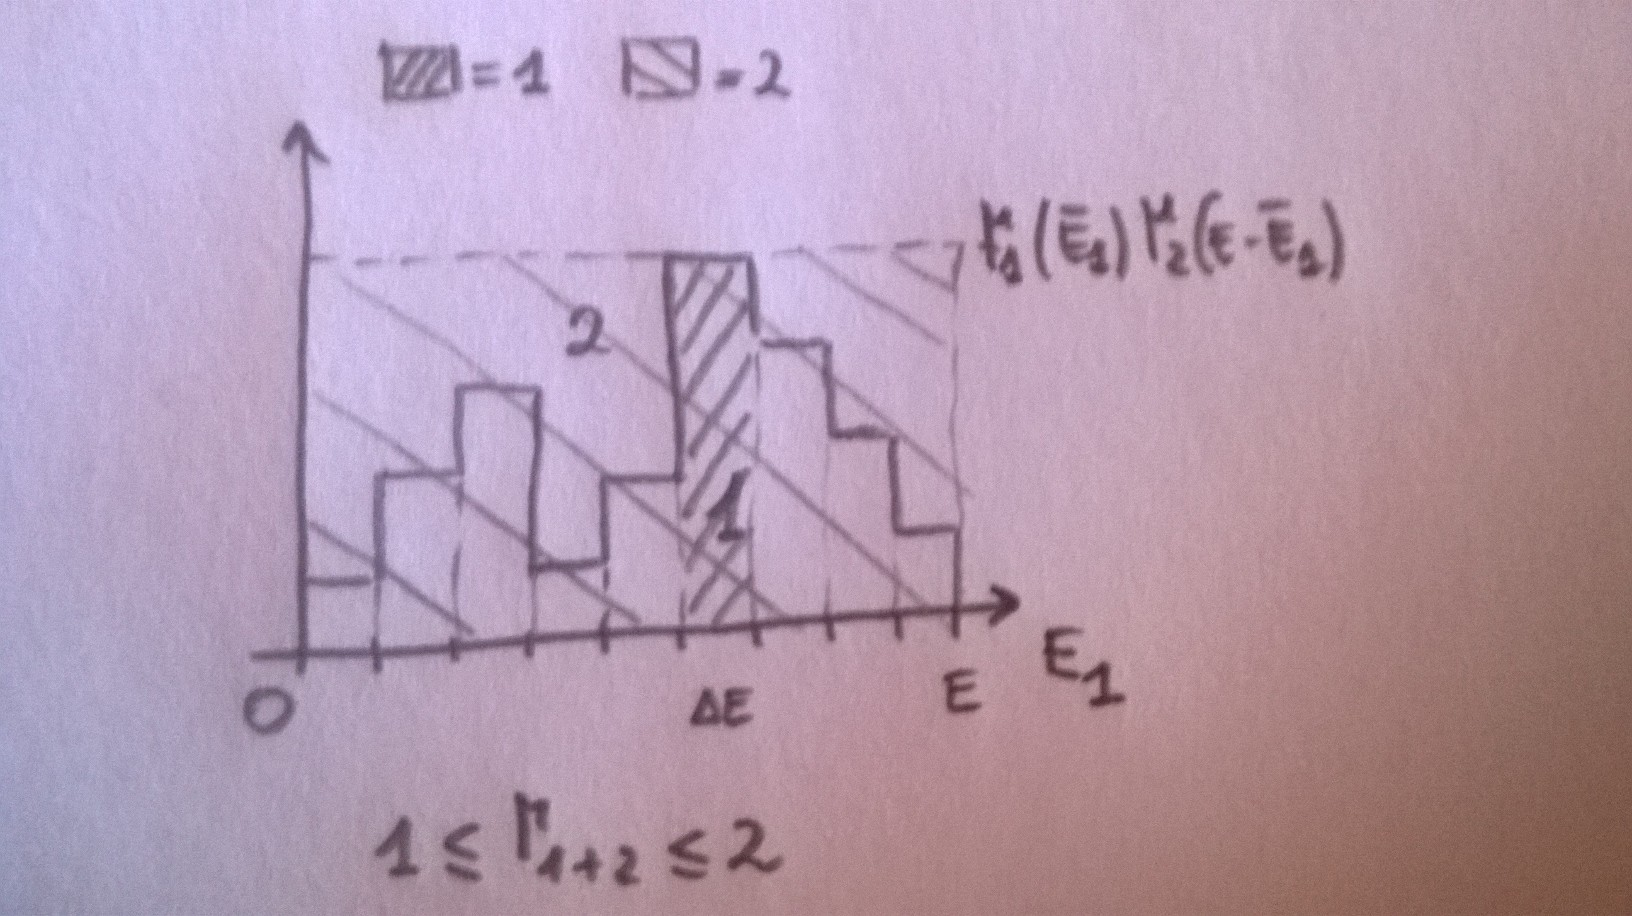
\includegraphics[width=100mm]{figure5.jpg}
\end{figure}

Since logarithm is a monotonically increasing function, I can apply it:

$$ln(\Gamma_1(\bar{E_1})\cdot \Gamma_2(E- \bar{E_1})) \le ln(\Gamma_{1+2}) \le ln(\Gamma_1(\bar{E_1})\cdot \Gamma_2(E-\bar{E_1}) \cdot \frac{E}{\Delta E})$$

using logarithm properties:

$$ln(\Gamma_1(\bar{E_1})) + ln(\Gamma_2(E- \bar{E_1})) \le ln(\Gamma_{1+2}) \le ln(\Gamma_1(\bar{E_1})) + ln(\Gamma_2(E-\bar{E_1})) + ln(E) - ln(\Delta E)$$

multiplying by $K_B$:

$$S_1(\bar{E_1}) + S_2(E-\bar{E_1}) \le S_{1+2}(E) \le S_1(\bar{E_1}) + S_2(E-\bar{E_1}) + K_B ln(E) - K_B ln(\Delta E)$$

Using \textit{squeeze theorem}, we take the limit for $N \to \infty$. Volume in phase space increases exponentially with N, this means that entropy grows linearly with N. The last two terms are negligible as $N \to \infty$ with respect to entropies, because $K_B ln(E) \to ln(N)$ and $K_B ln(\Delta E)$ is a constant independent of N. So:

$$S_1(\bar{E_1}) + S_2(E-\bar{E_1}) \le S_{1+2}(E) \le S_1(\bar{E_1}) + S_2(E-\bar{E_1})$$

that implies:

$$S_{1+2}(E) = S_1(\bar{E_1}) + S_2(E- \bar{E_1})$$

which proves the extensive property of the entropy. Actually we have proven also that system one can take any value of energy, but choose to spend the most of the time in $\bar{E_1}$, that is the value of energy that maximizes the product $\Gamma_1(E_1)\Gamma_2(E_2)$.\newline
This means that $\bar{E_1}$ is the value that makes the product stationary:

$$\left [ \frac{\partial}{\partial E_1} \Gamma_1(E_1)\Gamma_2(E-E_1) \right ]_{\bar{E_1}}= 0$$

making the derivative and using $\partial E_2 = - \partial E_1$:

$$\left [ \Gamma_2(E_2) \frac{\partial}{\partial E_1} \Gamma_1(E_1) \right ]_{\bar{E_1}} - \left [ \Gamma_1 (E_1) \frac{\partial}{\partial E_2} \Gamma_2(E_2) \right ]_{\bar{E_1}} = 0$$

so we find an equation that describes the condition for equilibrium, in which left hand side depends only on properties of system 1 and right hand side from properties of system 2:

$$\left [ \frac{1}{\Gamma_1(E_1)} \frac{\partial}{\partial E_1} \Gamma_1(E_1) \right ]_{\bar{E_1}} = \left [ \frac{1}{\Gamma_2 (E_2)} \frac{\partial}{\partial E_2} \Gamma_2(E_2) \right ]_{\bar{E_1}}$$

\paragraph{A second definition of entropy}

We now want to demonstrate that summing states on $0 \le H \le E$ or $E \le H \le H + \Delta$ is the same.\newline
\textbf{Claim:}

$$S_{\Delta}(E) = k_B ln (\int_{E \le H \le H + \Delta} d^{6N} \Gamma) =k_B ln (\int_{0 \le H \le E} d^{6N} \Gamma)$$

\textbf{Proof:} with analogous procedure as before

$$\Gamma_{\Delta}(\bar{E}) \le \sum_{i=0}^{E/\Delta} \Gamma_{\Delta}(E_i) \le \Gamma_{\Delta}(\bar{E}) \cdot \frac{E}{\Delta}$$

\begin{figure}[H]
\centering
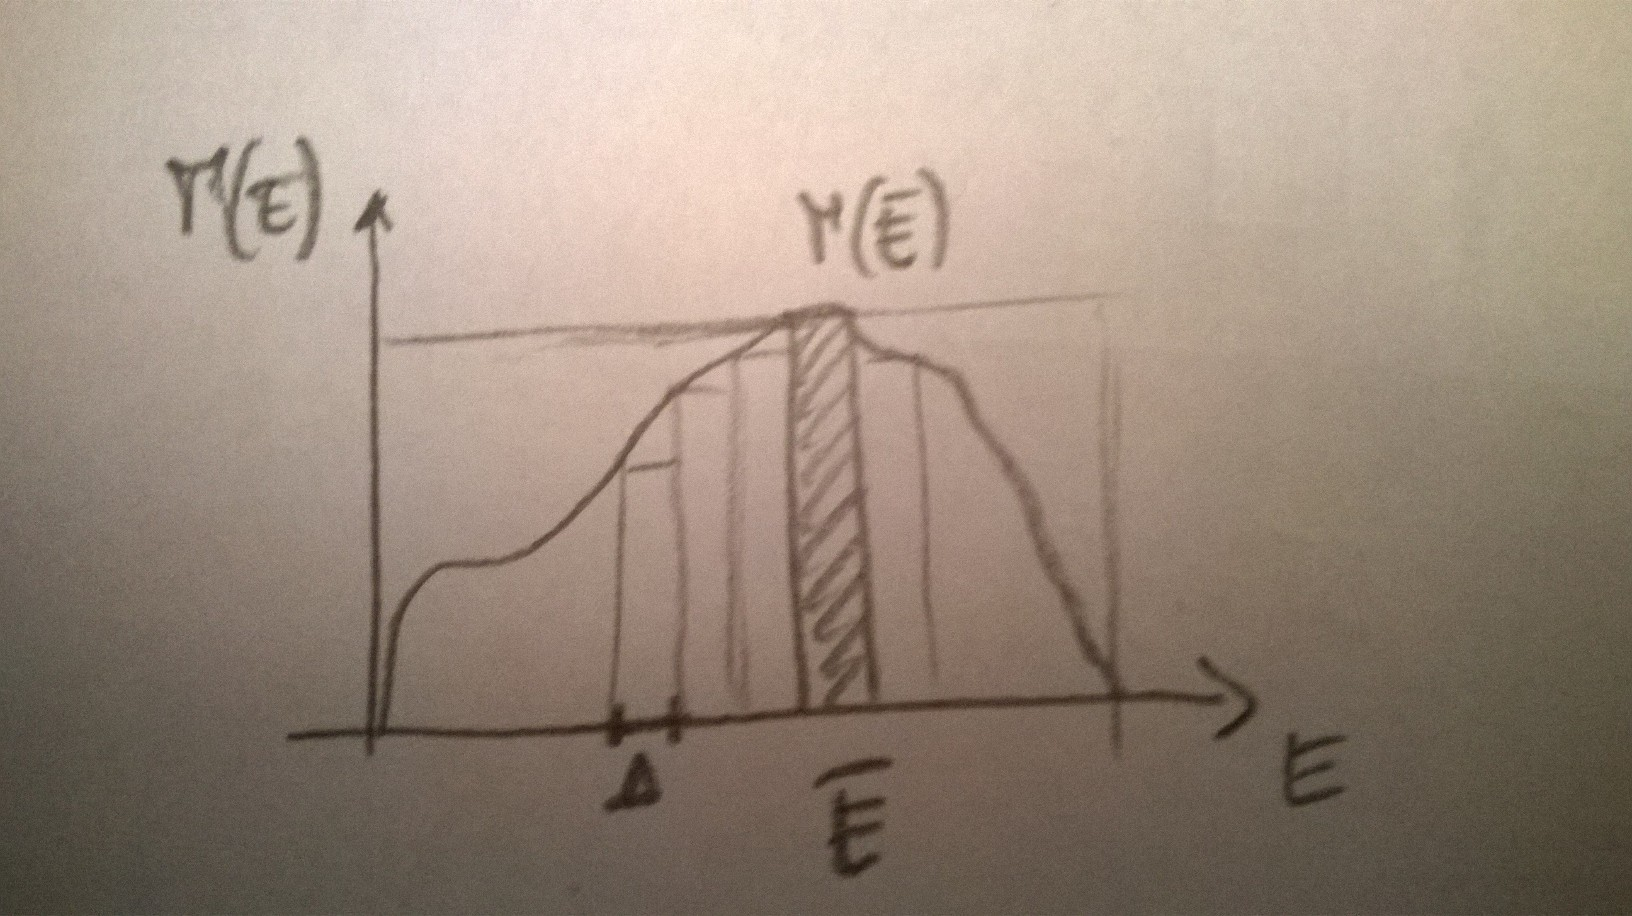
\includegraphics[width=100mm]{figure6.jpg}
\end{figure}

taking the logarithm of each member and multiplying by $k_B$ (monotonically increasing function and positive number, so we are allowed):

$$S_{\mbox{1st def}}(\bar{E}) \le S_{\mbox{2nd def}}(E) \le S_{\mbox{1st def}}(\bar{E}) + k_B ln (E) - k_B ln(\Delta)$$

since $ln(E) \propto ln(N)$ and $ ln(\Delta) \propto \mbox{constant}$ as $N \to \infty$, while $S \propto N$, using squeeze theorem for the limit $N \to \infty$:

$$S_{\mbox{2nd def}}(E) = S_{\mbox{1st def}}(\bar{E})$$

For all reasonable systems the maximum of S is obtained at the largest value of energy, in this case the two definitions coincide. $\bar{E}$ is the value that makes $\Gamma(E)$ the largest and it's the maximum value of E. In other words $\Gamma(E)$ is an increasing function of E.

\textbf{N.B.}: a posteriori we can say that the volume of integration in the first definition of entropy is $\bar{E} \le H \le \bar{E} + \Delta$, but a priori we don't know that, so we use a more general notation.

We now derive the explicit expression of $S(E)$ from the second definition:

$$S(E) = k_B ln(\int_{0 \le H \le E}d^{6N}\Gamma) = k_B ln \left [ \int d^{3N}q \int_{0 \le \sum_i |p_i|^2 \le 2mE} d^{3N}p \right ] = k_B ln \left [ V^N (2mE)^{3N/2} \cdot c_{3N} \right ]$$

where $c_{3N} = \frac{3N}{2} ln\pi - \frac{3N}{2} ln \frac{3N}{2} + \frac{3N}{2} + \mbox{higher order terms}$.\newline 
Taking the partial derivative in energy:

$$\frac{\partial S(E)}{\partial E} = \frac{3}{2} N k_B E^{-1}$$

Experimentally 

$$E = \frac{3}{2} N k_B T$$

so:

$$\frac{\partial S(E)}{\partial E} = \frac{1}{T}$$

If $\Gamma(E)$ is an increasing function of E, its logarithm will be and $S(E)$ will be an increasing function too.\newline 
Its partial derivative in E will be positive, so $T > 0$.

\paragraph{Laser - Different behavior of S and T}

\begin{figure}[H]
\centering
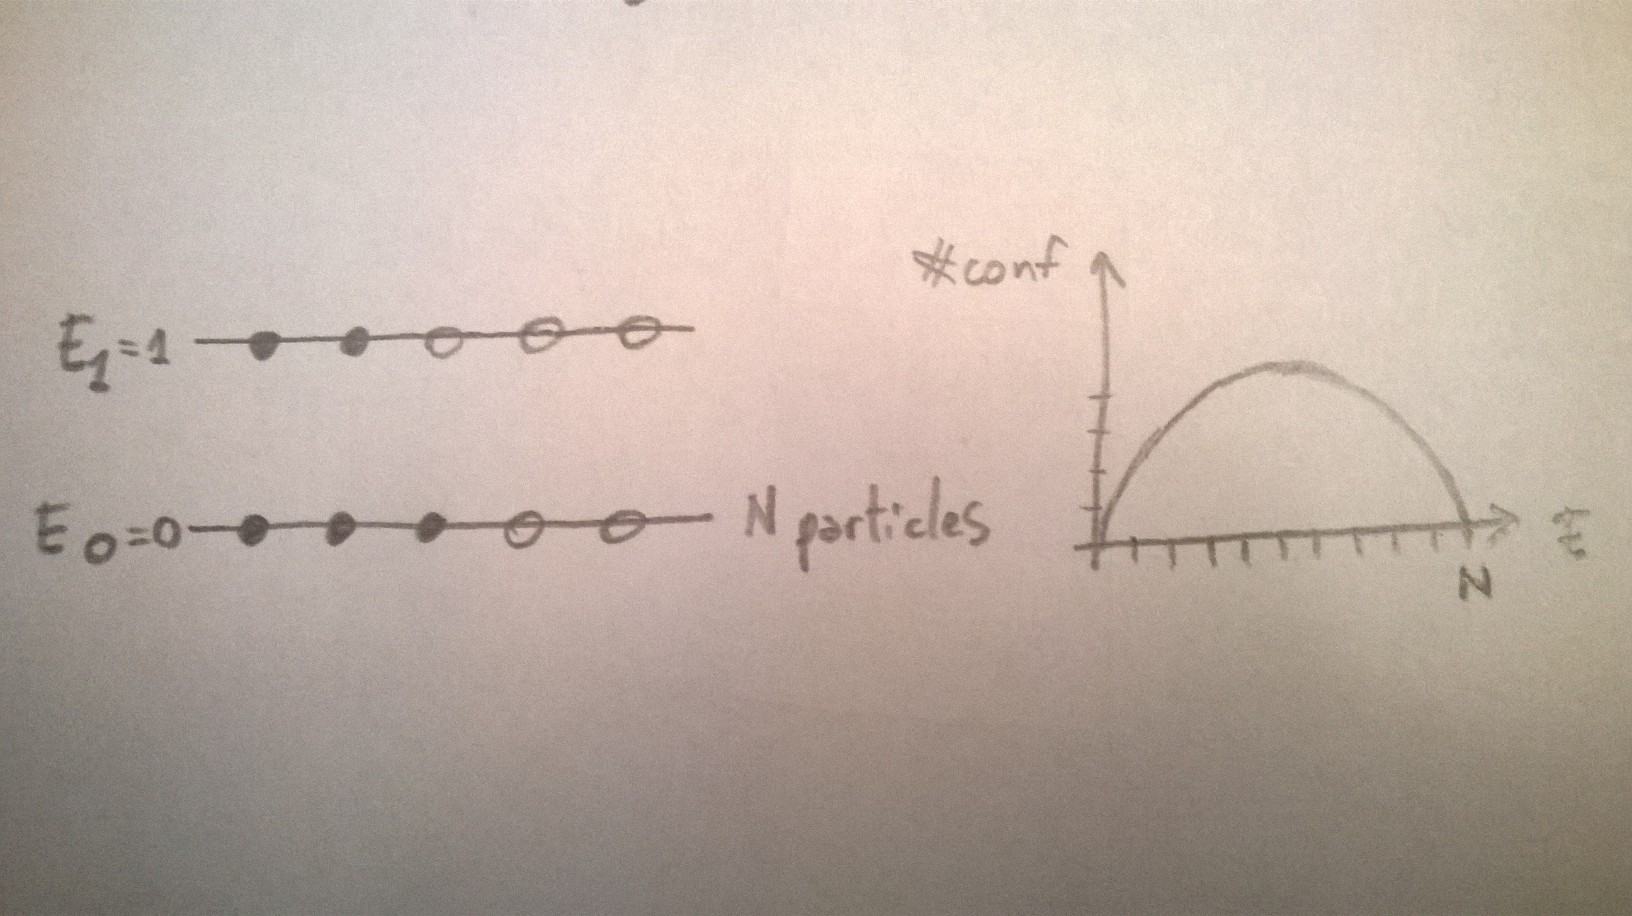
\includegraphics[width=140mm]{figure7.jpg}
\end{figure}

$\Gamma (E)$ is a non monotonic function of E. In this case, until $\tilde{E}$ is reached, T is rising, at $\tilde{E}$ $T \to \infty$, then $T<0$ (figure above).

\paragraph{Phase transitions}

In some situations if I plot E vs T, I get that one slope touches three points, it's a \textbf{phase transition}.

\begin{figure}[H]
\centering
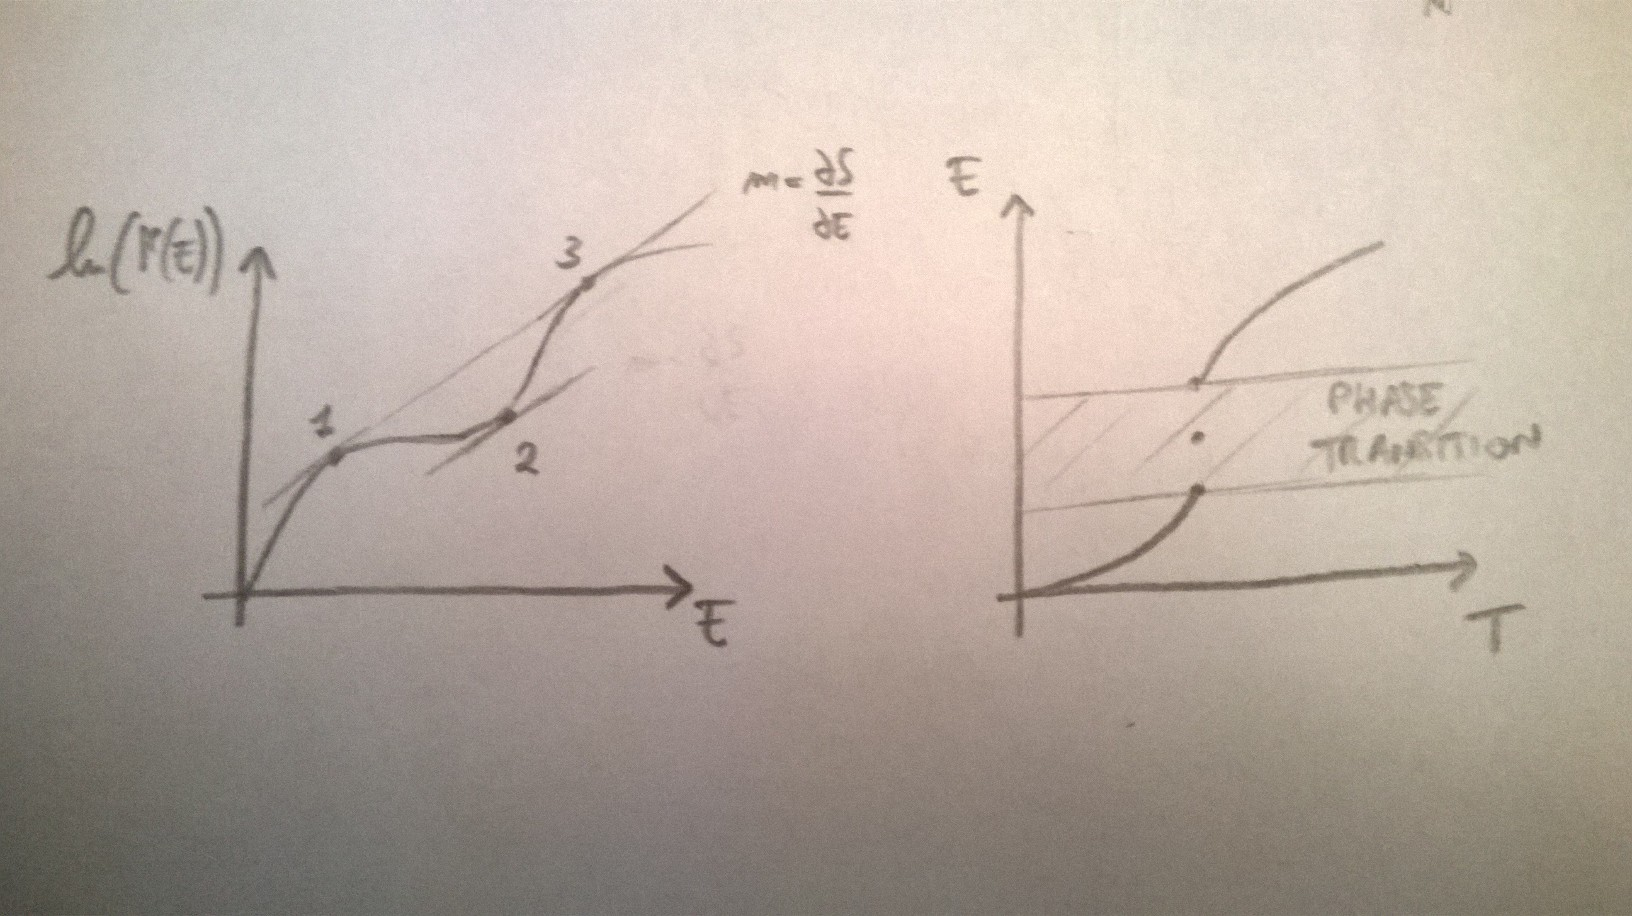
\includegraphics[width=100mm]{figure8.jpg}
\end{figure}

\paragraph{Computing observables}

Any observable can be computed as time average or:

$$<A> = \frac{\int d^{6N}\Gamma \rho(\overrightarrow{q}, \overrightarrow{p})\cdot A(\overrightarrow{q}, \overrightarrow{p})}{\int d^{6N}\Gamma \rho(\overrightarrow{q}, \overrightarrow{p})}$$

$S = k_B ln(\Gamma_\Delta (E))$ is not a definition like that, we can define it in a more compliant way (\textit{Shannon Entropy}):

$$S \propto - \int d^{6N} \Gamma \rho(\overrightarrow{q}, \overrightarrow{p}) \cdot ln( \rho(\overrightarrow{q}, \overrightarrow{p})$$

\subsection{Computing $\rho$}

Given this definition of entropy, we have to maximize the functional $F\left [ \rho \right ]$, in order to find $\rho*$ that makes it stationary. To simplify notation: $d^{6N}\Gamma = d\Gamma$.

$$F \left [ \rho \right ] = -k_B \int d\Gamma \left [ \rho ln(\rho) \right ]$$

with conditions:

$$\begin{cases}
\int d\Gamma \rho(q, p) = 1\\
\rho(q, p) = 0 \mbox{ if } H(q, p) \in \left [ E, E+\Delta E \right ]
\end{cases}
$$

We use \textbf{Lagrange multipliers}:

$$F\left [ \rho \right ] = -k_B \int d\Gamma \left [ \rho ln(\rho) -\lambda \rho \right ]$$

If we find solution $\rho^*$ and introduce a pointwise perturbation $\Delta \rho$, then we won't have linear dipendence of $\Delta F$ from $\Delta \rho$, but $\Delta F \propto (\Delta \rho^2)$.

$$\delta F = F[\rho +\Delta \rho] - F[\rho]$$ 

if I'm dealing with $\rho^*$ that maximizes F, in the limit $\frac{\rho}{\Delta\rho}$ small:

$$F[\rho^* +\Delta \rho] - F[\rho^*] = \Delta \rho^2 \mbox{ or higher order terms}$$ 

$$\delta F = -k_B \int d\Gamma \left \{ (\rho + \delta \rho)ln(\rho + \delta \rho) - \lambda (\rho +\delta \rho) - [\rho ln \rho -\lambda \rho] \right \}$$

given $ln(\rho + \delta \rho) \sim ln\rho + \frac{\delta \rho}{\rho} + \mbox{ higher order terms}$, that is a "generalization of Taylor expansion to functionals":

$$\delta F = - k_B \int d\Gamma \left \{ \rho ln\rho + \delta \rho + \delta \rho ln \rho - \lambda \delta \rho - \rho ln \rho \right \} = -k_B \int d\Gamma \left \{ \delta \rho [(1-\lambda) + ln \rho ] \right \}$$

if we are dealing with $\rho^*$, then the first order term in $\delta \rho$ needs to disappear, so, since we can choose $\delta \rho$ in an arbitrary way, we have to annihilate the integrand:

$$ln(\rho^*(q, p)) + 1-\lambda = 0 \mbox{ for all q, p compatible with } E \le H \le E+ \Delta E$$

then:

$$\rho^*(q, p) = e^{\lambda -1} = \mbox{constant}$$

\section{Canonical Ensemble}

\subsection{Computing $\rho$}

Now our constraint is that the \textbf{average energy of the system is constant}. Our conditions are:

$$\begin{cases}
\int d\Gamma \rho(q, p) = 1\\
\int d\Gamma \rho(q, p) H(q, p) = <H> = \bar{E}
\end{cases}
$$

Again we take the functional and maximize it with Lagrange multipliers (this time $\lambda$ and $\beta$). The calculation is very similar as before and we use always $\rho ln \rho \sim ln\rho + \frac{\delta \rho}{\rho}$:

$$\delta F = -k_B \int d\Gamma \left \{ \delta \rho [(1-\lambda) + ln \rho + \beta H] \right \}$$

for the same reason as before:

$$ln(\rho^*) + 1 - \lambda + \beta H = 0$$

then

$$\rho^* = e^{\lambda -1 -\beta H} \propto e^{-\beta H}$$

that is the result for the \textbf{canonical ensemble}. Actually we find:

$$\rho^* = \frac{e^{-\beta H}}{\int d\Gamma e^{-\beta H}}$$

\paragraph{Physical meaning of $\beta$}

$$<H> = \frac{\int d\Gamma H e^{-\beta H}}{\int d\Gamma e^{-\beta H}} = -\frac{\partial}{\partial \beta} \left [ ln \int d\Gamma e^{-\beta H} \right ] = -\frac{\partial}{\partial \beta} ln \mathcal{Z}$$

In an ideal gas $H = \sum_i \frac{p_i^2}{2m}$:

$$\mathcal{Z} = \int d^{3N} q \int d^{3N} p e^{- \beta \sum_i \frac{p_i^2}{2m}} = V^N \left [ \int dp e^{-\beta \frac{p^2}{2m} }\right ]^{3N}$$

that is a gaussian integral, given:

$$\int dx e^{-\frac{x^2}{2\sigma^2}} = \sqrt{2\pi \sigma^2}$$

we have:

$$\mathcal{Z} = V^N \left ( 2\pi \frac{m}{\beta} \right )^{\frac{3N}{2}}$$

taking the logarithm of $\mathcal{Z}$, doing its derivative in $\beta$ and then multiplying by a minus sign:

$$<H> = \frac{3}{2}\frac{1}{\beta}$$

experimentally:

$$<H> = \frac{3}{2}\frac{1}{\beta} = \frac{3}{2} N k_B T$$

so $\beta = \frac{1}{k_B T}$


\subsection{Fluctuation and dissipation relationship}

If we take the second derivative of $ln\mathcal{Z}$ in $\beta$, we have:

$$\frac{\partial^2}{\partial \beta^2} ln \mathcal{Z} = - \frac{\partial}{\partial \beta} \left ( -\frac{\partial}{\partial \beta} ln\mathcal{Z} \right ) = -\frac{\partial}{\partial \beta} \frac{\int d\Gamma H e^{-\beta H}}{\int d\Gamma e^{-\beta H}} = \frac{\int d\Gamma H^2 e^{-\beta H} \mathcal{Z} - \int d\Gamma H e^{-\beta H} \int d\Gamma H e^{-\beta H}}{\left ( \int d\Gamma e^{-\beta H} \right )^2} =$$
$$= \frac{\int d\Gamma H^2 e^{-\beta H}}{\mathcal{Z}} - \left (\frac{ \int d\Gamma H e^{-\beta H}}{\mathcal{Z}}\right )^2 = <H^2> - <H>^2$$

but, since $d\beta = -\frac{1}{k_B T^2} dT$

$$\frac{\partial^2}{\partial \beta^2} ln \mathcal{Z} = -\frac{\partial}{\partial \beta} <H> = k_B T^2 \frac{\partial <H>}{\partial T}$$

and $c_v = \frac{\partial <H>}{\partial T}$ is the specific heat. So we've found:

$$<H^2> - <H>^2 = k_B T^2 \frac{\partial <H>}{\partial T}$$

a relationship between an equilibrium property on the left and a something that depends on how energy of the system varies changing T. This is called \textbf{fluctuation and dissipation relationship}

We have

$$\frac{\Delta E}{E} = \sqrt{\frac{<H^2> -<H>^2}{<H>^2}} \propto \sqrt{N/N^2} = \frac{1}{\sqrt{N}}$$

as $N \to \infty$, $\frac{\Delta E}{E} \to 0$

while

$$\Delta E \propto \sqrt{N}$$

so the absolute displacement increases, but the relative displacement tends to 0.

\begin{figure}[H]
\centering
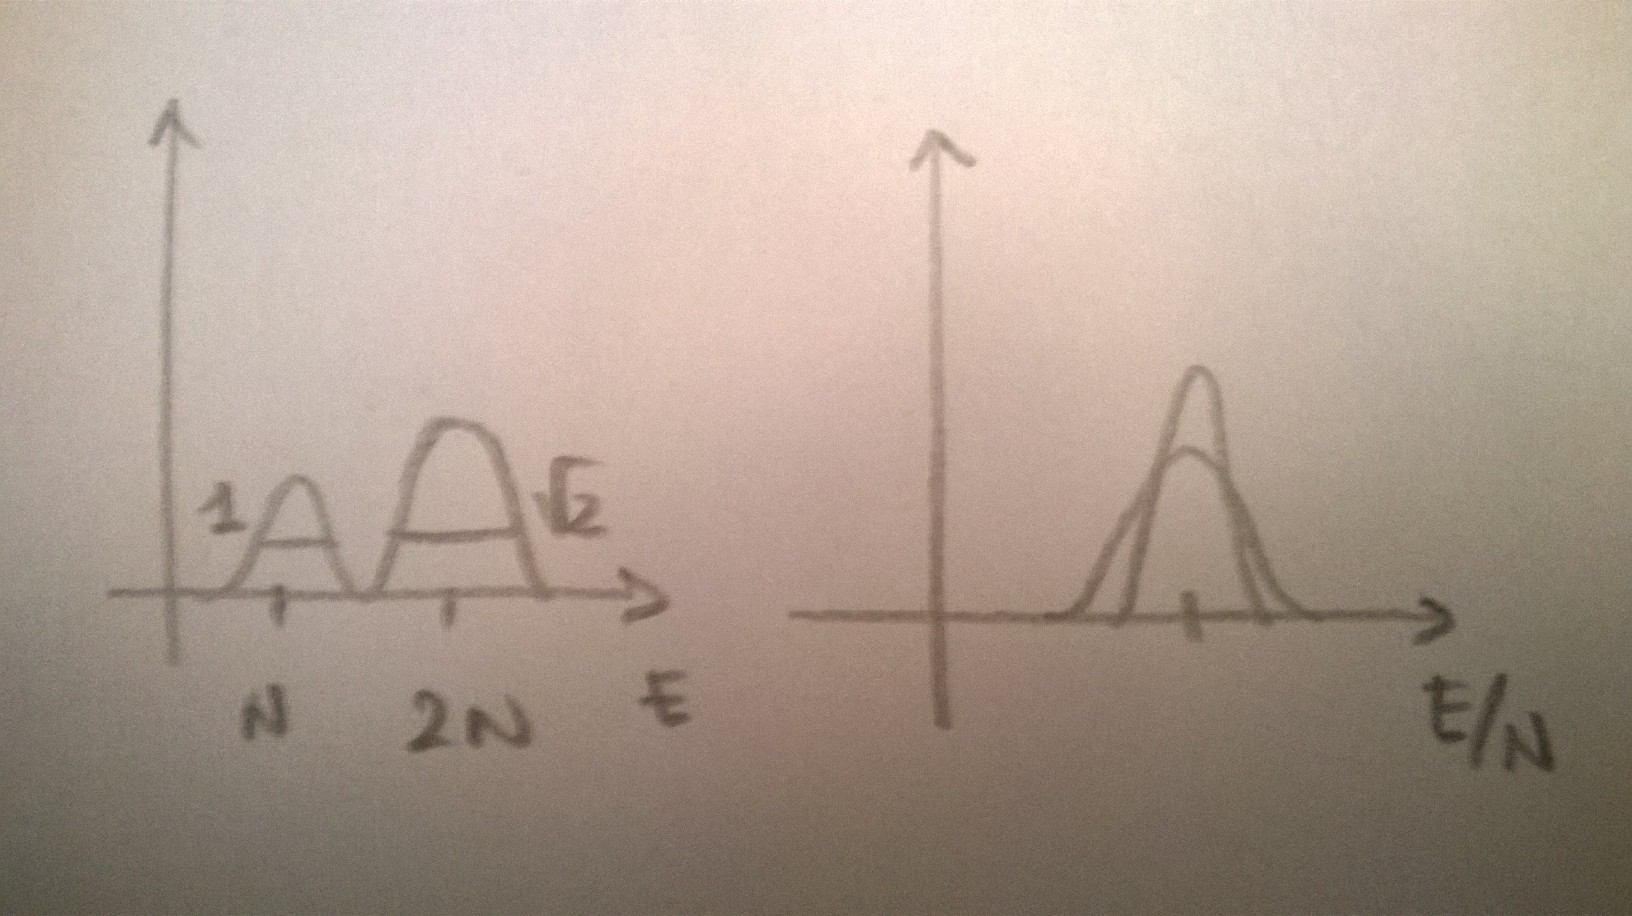
\includegraphics[width=100mm]{figure9.jpg}
\end{figure}

\subsection{Helmholtz Free Energy}

If we compute the entropy with the $\rho$ we found:

$$S = -k_B \int d\Gamma \rho(q, p) ln \rho(q, p) = -k_B \int d\Gamma \frac{e^{-\beta H}}{\mathcal{Z}} (-\beta H --ln \mathcal{Z}) = k_B \beta <H> + k_B ln \mathcal{Z}$$

multiplying both sides by T:

$$- k_B T ln \mathcal{Z} = <H> - TS$$

We finally find:

$$F = U - TS = \mbox{free energy}$$

so $\mathcal{Z} = e^{-\beta F}$: the canonical partition function is related to the free energy of the system.

$$\mathcal{Z} = N k_B T ln \left [ V (\frac{2\pi m}{\beta})^{3/2} \right] + \frac{3}{2} N k_B T$$

$$F = -\frac{1}{\beta} \left [ N ln V + \frac{3}{2} N ln(2\pi m) - \frac{3}{2} N ln \beta \right ]$$

If we did things in the right way, we should find $- \frac{\partial F}{\partial V} = \mbox{pressure} = p$, check:

$$- \frac{\partial F}{\partial V} = \frac{1}{\beta} \frac{N}{V} = \frac{N k_B T}{V} = p$$

that is correct.

\paragraph{Disturbing fact}

We have two systems, with the same density and the same temperature.

$$\frac{N_1}{V_1} = \frac{N_2}{V_2}$$

If I put them in contact and I don't allow flow of particles, nothing forbids me to look at the system $N_1 + N_2, V_1 + V2$, but I find $S_{TOT} - (S_1 + S_2) = (N_1 + N_2) ln(V_1 + V_2) - N_1 ln V_1 - N_2 ln V_2 \ne 0$ in general. This is known as \textbf{Gibbs paradox}. There's a problem related to the dependence of S from N. This will be solved by \textbf{correct Boltzmann counting}: whenever integrating over phase space, we should add a factor $\frac{1}{N!}$ (further information on paper by Robert H. Swendsen, \textit{Gibbs' Paradox and the Definition of Entropy}, Carnegie Mellon University).

$$\int d\Gamma \rightarrow \frac{1}{N!}\int d\Gamma$$

This factor reduces the counting of the states. It is an \textbf{ad hoc correction}. When computing the entropy:

$$S^{correct} = S - ln(N!) \simeq S - Nln(N) $$

where we have used Stirling approximation. With this definition of entropy:

$$S_{1+2}^{correct} = S_{1+2} - (N_1+N_2)ln(N_1+N_2)$$

$$S_{1}^{correct} + S_2^{correct} = S_1 + S_2 - N_1ln(N_1) - N_2 ln(N_2)$$

so

$$S_{1+2}-(S_{1}+S_{2}) = N_1 ln \left ( \frac{V_1+V_2}{N_1+N_2} \right ) - N_1 ln \left ( \frac{V_1}{N_1} \right ) - N_2 ln \left ( \frac{V_2}{N_2}\right )$$

given that arguments of logarithms are the densities and they are all equal, we have $S_{1+2}-(S_{1}+S_{2}) = 0$, which is correct.

\section{Grand canonical ensemble}

In the grand canonical ensemble we have $<N>$ fixed, but N can vary, so we have $6N+1$ degrees of freedom.

$$S = -k_B \sum_N \int d\Gamma \rho_N ln \left ( \rho_N \right )$$

\textbf{CONSTRAINTS}:
\begin{itemize}
\item $\sum_N \int d\Gamma \rho_N =1 \rightarrow \lambda$
\item $\sum_N \int d\Gamma \rho_N H = \bar{E} \rightarrow \beta$
\item $\sum_N \int d\Gamma \rho_N N = \bar{N} \rightarrow \beta \mu$
\end{itemize}

In order to find $\rho$ of the grand canonical ensemble, we maximize S.

$$\tilde{F} = - k_B \sum_N \int d\Gamma \rho_N \left [ ln\left ( \rho_N \right ) + \lambda + \beta H_n - \beta \mu n \right ]$$

We are adding a linear term in $\delta \rho$, so when we do the functional derivative and put it equal zero, we get:

$$\delta \tilde{F} = 0 = -k_B \sum_N \int d\Gamma \delta \rho \left [ ln \left ( \rho \right ) + 1 + \lambda + \beta H - \beta \mu N\right ]$$

This should be true, no matter the choice of $\delta \rho$, so the integrand must be zero and we get:

$$\rho^* =  \frac{e^{-\beta\left [ H_N - \mu N \right ]}}{\mathcal{Z}}$$

$$\mathcal{Z} = \sum_N \frac{1}{N!} \int d\Gamma e^{-\beta\left ( H_N - \mu N \right )} $$

We can define the free energy of the system by saying that:

$$\mathcal{Z} = e^{-\beta F}$$

and redefine 

$$\rho = \frac{e^{-\beta\left [ H_N - \mu N \right ]}}{e^{-\beta F}}$$

Computing the entropy:

$$S = -k_B \sum_N \int d\Gamma \rho ln(\rho) = k_B \sum_N \int d\Gamma \rho \left [ \beta(H_N - \mu N) -\beta F \right ] = k_B \left [ \beta <H> - \mu \beta <N> -\beta F \right ]$$

this means

$$S = \frac{\bar{E}}{T} - \frac{\mu \bar{N}}{T} - \frac{F}{T}$$

multiplying by T both sides and reorganizing terms:

$$\bar{F} = \bar{E} - \mu\bar{N} -TS$$

from this definition:

$$\mu = -\frac{\partial F}{\partial N}$$

$\mu$ is the chemical potential: energy associated with the introduction of one or more particles in the system. We have also:

$$\bar{N} = -\frac{\partial F}{\partial \mu}$$

We can check this:

$$ln \mathcal{Z} = -\beta F \rightarrow F = -\frac{1}{\beta} ln(\mathcal{Z})$$

and

$$\frac{\partial F}{\partial \mu} = \frac{1}{\beta \mathcal{Z}} \frac{\partial \mathcal{Z}}{\partial \mu}$$

given that $\mathcal{Z} \propto \sum_N \int d\Gamma e^{-\beta\left [ H_N - \mu N \right ]}$:

$$\frac{\partial \mathcal{Z}}{\partial \mu} \propto \sum_N \int d\Gamma e^{-\beta \left [ H_N - \mu N \right ]} \beta N \rightarrow -\frac{\partial F}{\partial \mu} = <N>$$

Differentiating F with respect to one of the intensive thermodynamic quantities returns the average value of its conjugate quantity. F is a thermodynamic potential.

\subsection{Ideal gas}

$$\mathcal{Z}_{grand canonical} = \sum_N \frac{1}{N!} \int d\Gamma e^{-\beta\left [ H_N - \mu N \right ]} = \sum_N \frac{1}{N!} e^{-\beta \mu N} \int d\Gamma e^{-\beta H_N}$$

This is equal to:

$$\mathcal{Z} = \sum_N \frac{1}{N!} e^{\beta \mu N} \left [ V^N \left ( \frac{2\pi m}{\beta} \right )^{\frac{3N}{2}} \right ] = \sum_N \frac{1}{N!} x^N = e^x$$

where $x = e^{\beta \mu} V \left ( \frac{2\pi m}{\beta} \right )^{\frac{3}{2}}$ and $e^{\beta \mu}$ is called \textit{fugacity}.\newline
We usually deal with $log\mathcal{Z}$, that is:

$$ln \mathcal{Z} = z V \left ( \frac{2\pi m}{\beta} \right )^{\frac{3}{2}}$$

$$<N> = - \frac{\partial F}{\partial \mu} = \frac{1}{\beta} \frac{\partial ln \mathcal{Z}}{\partial \mu} = e^{\beta \mu} V \left ( \frac{2\pi m}{\beta} \right )^{\frac{3}{2}}$$

so we find:

$$\frac{<N>}{V} = e^{\beta \mu} \left ( \frac{2 \pi m}{\beta}\right )^{\frac{3}{2}}$$

that is a relation between intensive quantities: density, fugacity, mass and temperature. Dependence on mass is particularly interesting: it comes from kinetic energy and is important to control equilibrium of chemical reactions.

\subsection{Derivation of law of mass action}

Let's take a chemical reaction as example:

$$2 H_2 + O_2 \leftrightarrow 2H_2 O$$

We want to know what are the fractions of each species of molecules in the mixture at equilibrium. More generally we consider a reaction:

$$ \nu_1 X_1 + \nu_2 X_2 + \ldots \leftrightarrow \nu'_1 Y_1 + \nu'_2 Y_2 + \ldots$$

where $\nu_i$ are called \textit{stoichiometric coefficients}, $X_i$ are \textit{volume concentrations}.\newline
Free energy has to be as little as possible at equilibrium and there are little fluctuations of N, since it is a dynamic equilibrium, however these fluctuations can not be arbitrary.

$$\partial F = \sum_i \frac{\partial F}{\partial N_i} \delta N_i = -\sum_i \mu_i \delta N_i = 0 \mbox{ at equilibrium}$$

so:

$$\sum_i \mu_i \delta N_i = 0$$

$\mu_i$ are known, but $\delta N_i$ are tricky: they can't be arbitrary, but must satisfy $\frac{\delta N_i}{\pm \nu_i} = \mbox{constant} = \delta n$. So we have:

$$\sum_i \mu_i v_i = \sum_j \mu_j v_j$$

where the right hand side refers to products and left hand side to reagents and this is the condition for equilibrium.\newline
If we take our first example:

$$2 \mu_{H_2} + 1\mu_{O_2} = 2\mu_{H_2O}$$

multiply both sides by $\beta$ and remember $\beta \mu = ln \left ( \left ( \frac{2\pi m}{\beta} \right )^{\frac{3}{2}} \frac{1}{V} \right )$:

$$2 ln \left ( \left ( \frac{2\pi m_{H_2}}{\beta} \right )^{\frac{3}{2}} \frac{1}{V_{H_2}} \right ) + ln \left ( \left ( \frac{2\pi m_{O_2}}{\beta} \right )^{\frac{3}{2}} \frac{1}{V_{O_2}} \right ) = 2ln \left ( \left ( \frac{2\pi m_{H_2O}}{\beta} \right )^{\frac{3}{2}} \frac{1}{V_{H_2O}} \right )$$

using properties of logarithms:

$$\frac{V_{H_2O}^2}{V_{H_2}^2V_{O_2}} \propto \frac{m_{H_2}^3 m_{O_2}^\frac{3}{2}}{m_{H_2O}^3}$$

that is the \textbf{law of mass action}. It is very important because shows that we can shift chemical equilibrium towards products or reagents by changing the mass (using isotopes). This comes from the kinetic contribution to the partition function $\mathcal{Z}$.

%%%%%%%%%%%%%%%
%MOLECULAR DYNAMICS%
%%%%%%%%%%%%%%%

\chapter{Molecular Dynamics}

\section{Hamilton Formalism}

$$q = \mbox{position}$$

$$\dot{q} = \mbox{velocity}$$

$$p = \mbox{momentum}$$

$$\dot{p} = \mbox{force}$$

These are all vectors of 3N components in the phase space (x, y, z components for each of N particles). \textbf{Hamilton equations}:

$$\begin{cases}
\dot{q} = \frac{\partial H }{\partial p} \\
\dot{p} = - \frac{\partial H}{\partial q}
\end{cases}$$

We make some \textbf{non general assumptions} on H, in order to be able to do computations:

$$H(q, p) = K(p) + U(q)$$

$$K(p) = \sum_i \frac{p_i^2}{2m_i}$$

that are: Hamiltonian is the sum of a term K depending only on p and a term U depending only on q; kinetic energy K is quadratic in p. With these assumptions we have:

$$\begin{cases}
\dot{q} = \frac{\partial K }{\partial p} = \frac{p}{m}\\
\dot{p} = - \frac{\partial U}{\partial q} = f
\end{cases}$$

that are two first order differential equations. Or we can state Newton Law:

$$\ddot{q} = \frac{f}{m}$$

that is a single second order differential equation.

\paragraph{Harmonic Oscillator}

\begin{figure}[H]
\centering
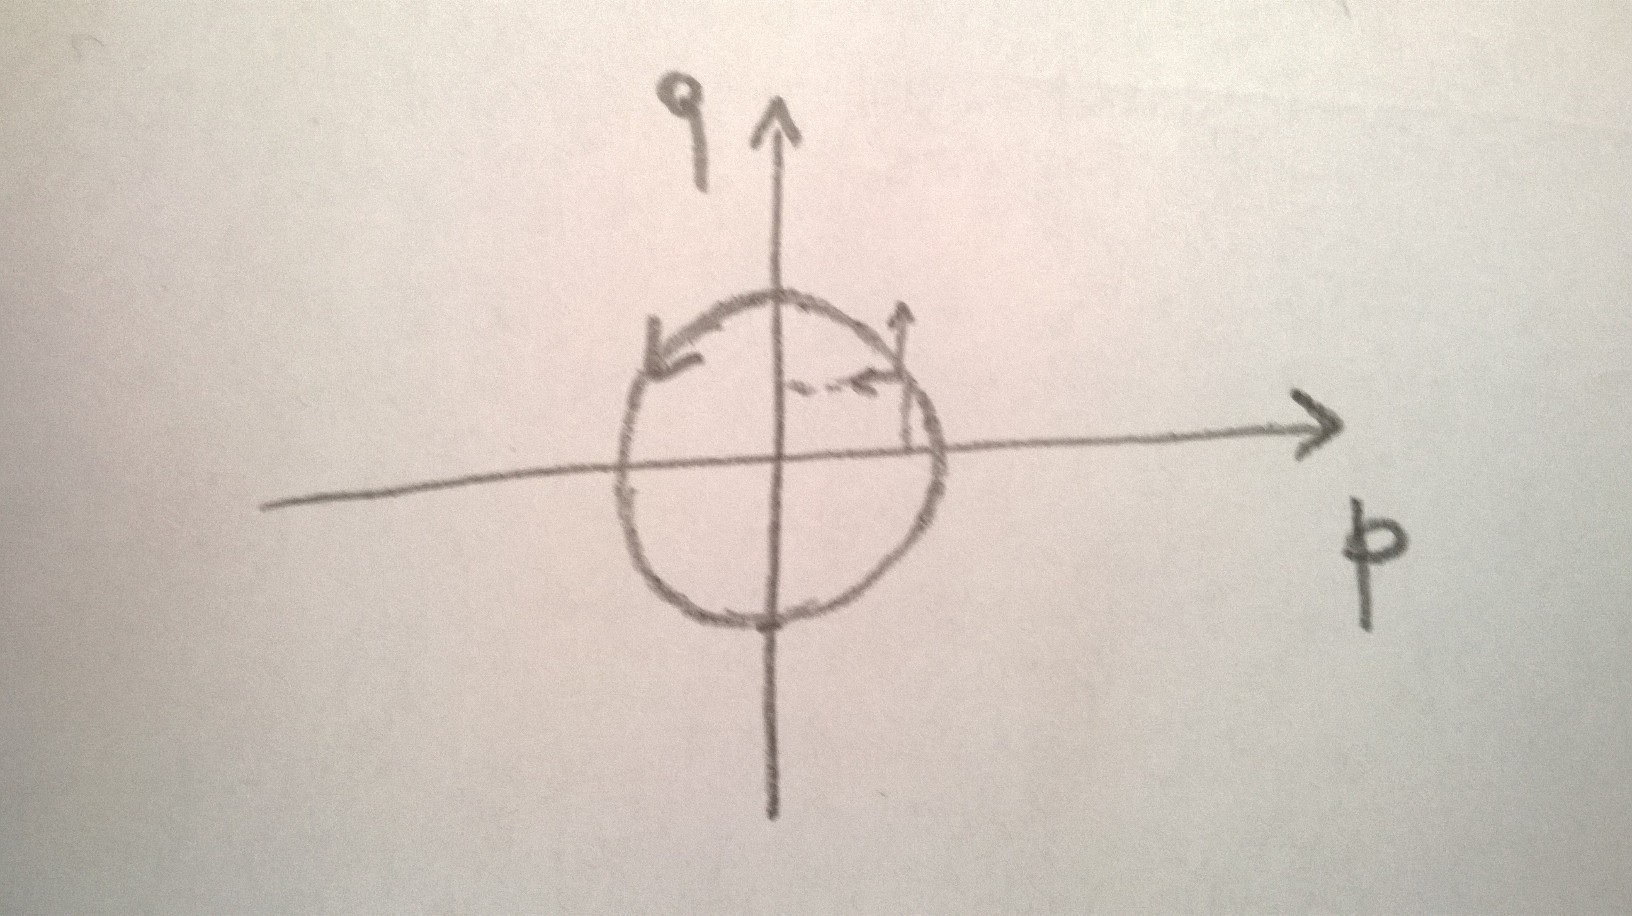
\includegraphics[width=100mm]{pic1.jpg}
\end{figure}

$$H = \frac{p^2}{2m} + \frac{1}{2} K q^2$$

if we assume $m=1$, $k=1$, then $H=\frac{p^2}{2} + \frac{q^2}{2}$ and

$$\dot{p} = -q$$
$$\dot{q} = p$$

\section{Liouville Formalism}

\begin{figure}[H]
\centering
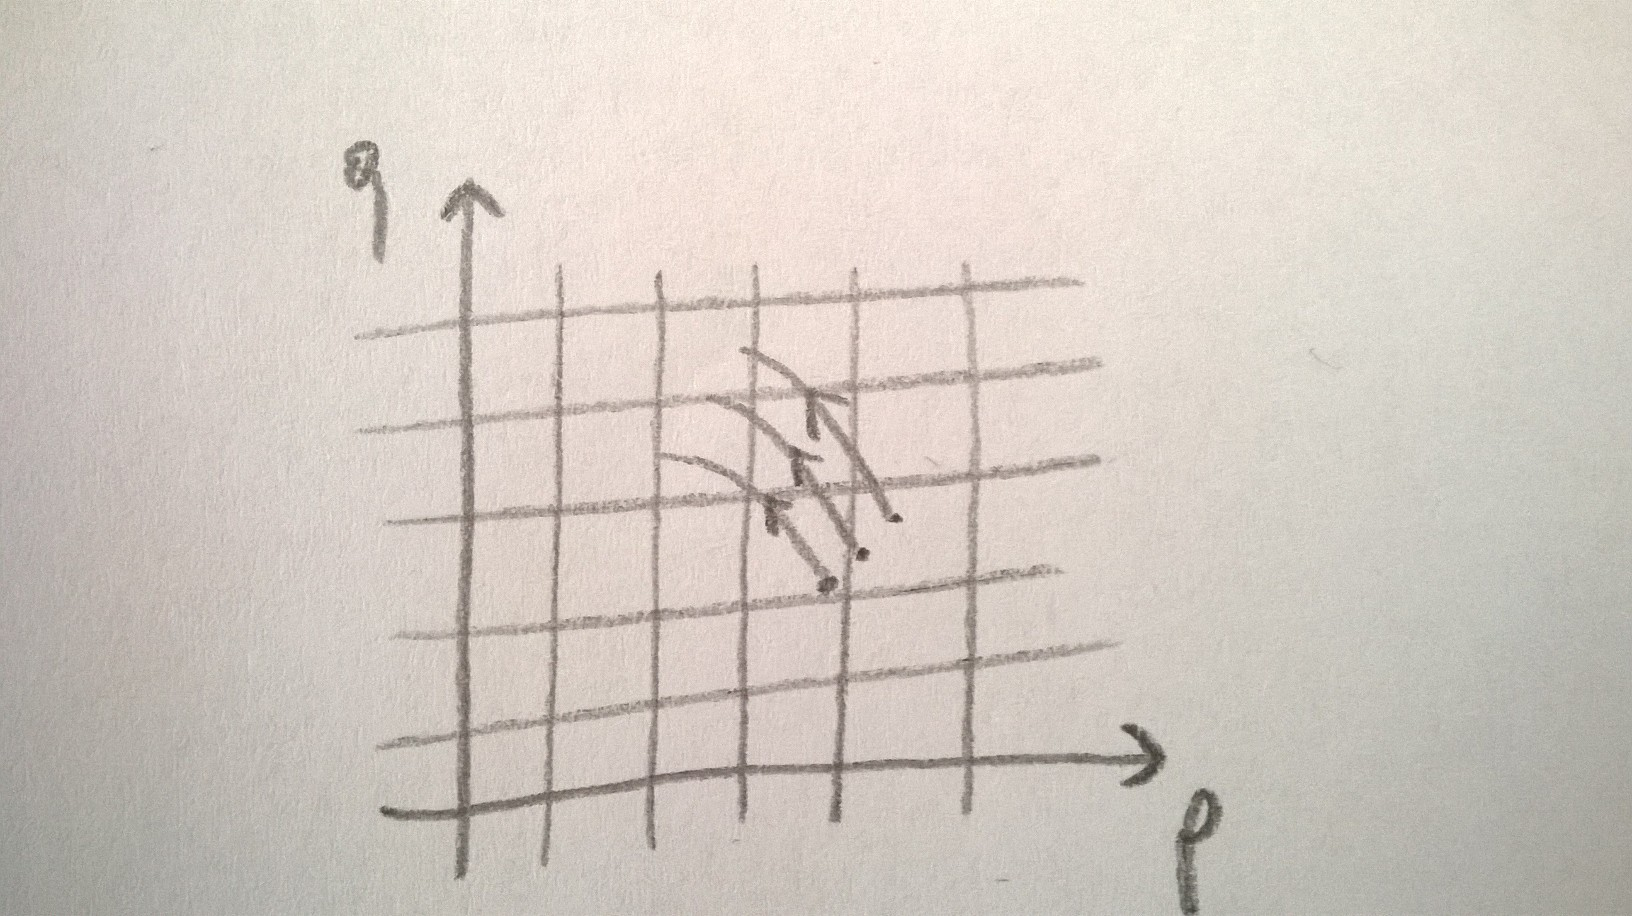
\includegraphics[width=100mm]{pic2.jpg}
\end{figure}

We define points $x = (q, p)$ and we can define a velocity $\dot{x}$, that is not the physical velocity, but the velocity of points in phase space.

$$\dot{x} = v(x)$$

then we can write:

$$\dot{\rho}(x, t) = - \overrightarrow{\nabla} \cdot \overrightarrow{J} (x, t) = - \overrightarrow{\nabla} \cdot (\rho \overrightarrow{v} ) = -\frac{\partial}{\partial p} (\rho \dot{p}) - \frac{\partial}{\partial q}(\rho \dot{q})$$

$$-\frac{\partial}{\partial p} (\rho \dot{p}) - \frac{\partial}{\partial q}(\rho \dot{q}) =  \frac{\partial}{\partial p} \left ( \rho \frac{\partial H}{\partial q} \right ) -  \frac{\partial}{\partial q} \left ( \rho \frac{\partial H}{\partial p} \right ) = \frac{\partial \rho}{\partial p} \frac{\partial H}{\partial q} + \rho \frac{\partial^2 H}{\partial q \partial p} - \frac{\partial \rho}{\partial q} \frac{\partial H}{\partial p} - \frac{\partial^2 H}{\partial q \partial p}$$

and finally:

$$\dot{\rho}(x, t) = \frac{\partial \rho}{\partial p} \frac{\partial H}{\partial q} - \frac{\partial \rho}{\partial q} \frac{\partial H}{\partial p} = - \hat{L} \cdot \rho$$

where $\hat{L}$ is called the \textbf{Liouville operator}.

$$\hat{L} = \hat{L_p} + \hat{L_q}$$

with $\hat{L_p} = -\frac{\partial H}{\partial q} \frac{\partial}{\partial p}$ and $\hat{L_q} = \frac{\partial H}{\partial p} \frac{\partial}{\partial q}$. If we solve $\dot{\rho} = - \hat{L} \rho$ we find:

$$\rho(t+\Delta t) = e^{-\Delta t \hat{L}} \rho(t)$$

that tells how an ensemble of trajectories evolves with time. If we take the total derivative of $\rho (x, t)$, we find:

\paragraph{Properties of trajectories}

\begin{itemize}
\item \textbf{Time reversal trajectory}: the time reversal trajectory satisfies the same Hamilton equation as the original one (requires non general assumptions we made before, it's not true in presence of a magnetic field for example).

$$(p(t), q(t)) \to (-p(-t), q(-t)) = (p*(t), q*(t))$$

$$\begin{cases}
\frac{\partial q*(t)}{\partial t} = \frac{\partial q(-t)}{\partial t} = - \frac{\partial q(-t)}{\partial (-t)} = - \frac{\partial  H}{\partial p} =  \frac{\partial  H}{\partial (-p)} =  \frac{\partial  H}{\partial p*}\\
\frac{\partial p*(t)}{\partial t} = - \frac{\partial p(-t)}{\partial t} = \frac{\partial p(-t)}{\partial (-t)} = - \frac{\partial  H}{\partial q} = - \frac{\partial  H}{\partial q*}
\end{cases}$$

\begin{figure}[H]
\centering
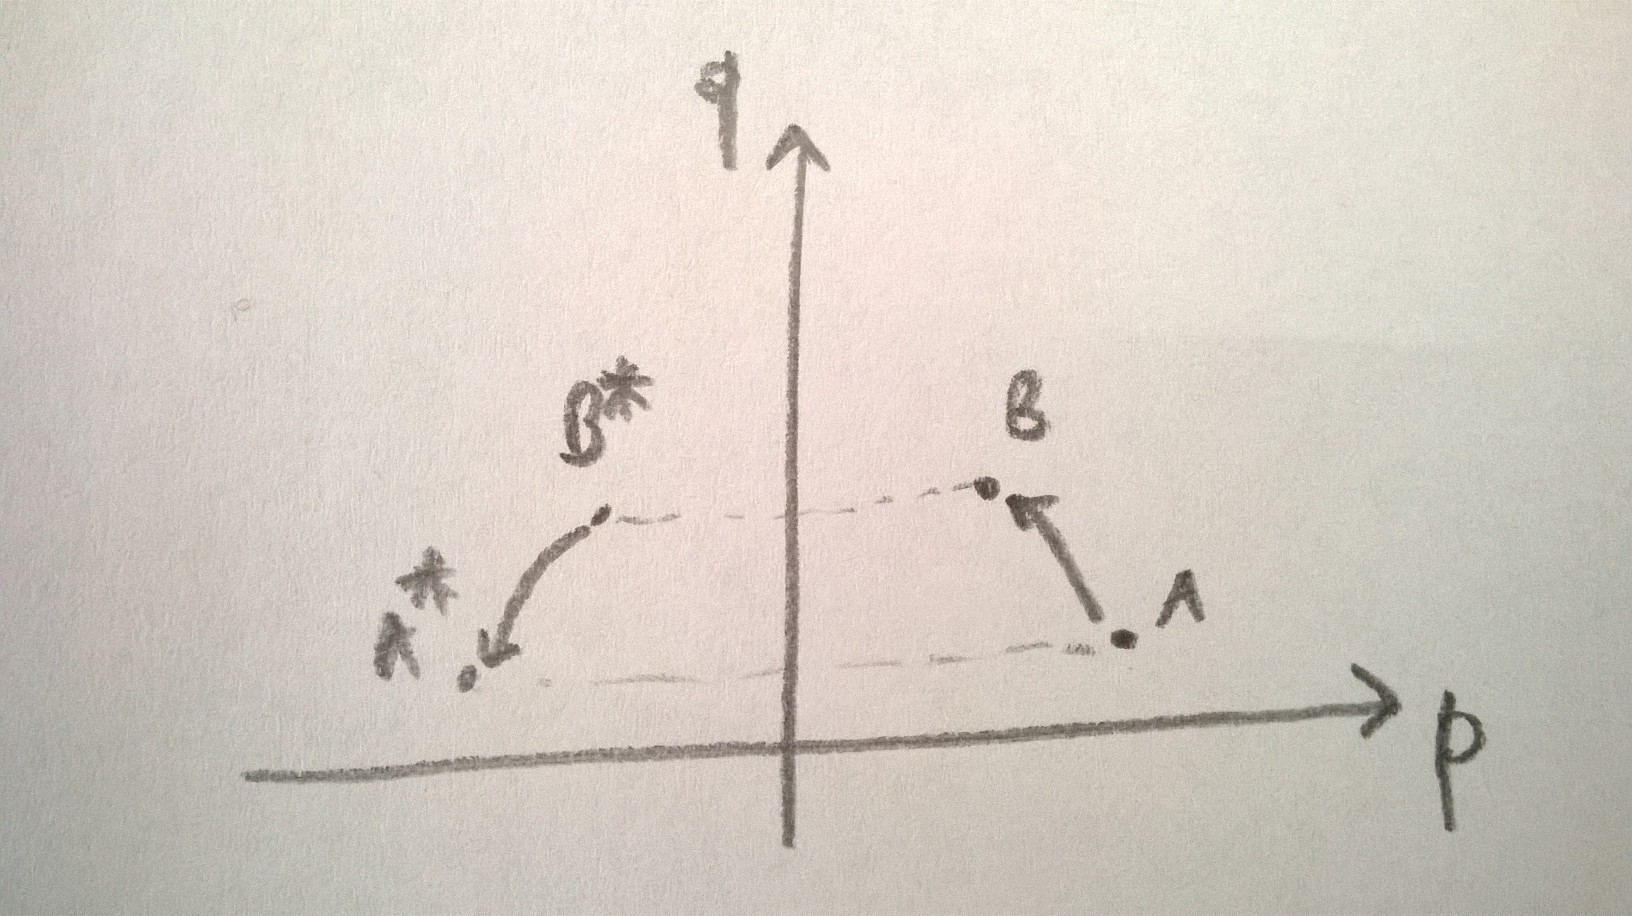
\includegraphics[width=100mm]{pic3.jpg}
\end{figure}

\item \textbf{Energy conservation}: we assume H depends on $t$ because of $p(t)$ and $q(t)$ and nothing else, then $\frac{\partial H}{\partial t} = 0$, so total derivative of H is:

$$\frac{dH}{dt} = \frac{\partial H}{\partial p} \frac{\partial p}{\partial t} + \frac{\partial H}{\partial q}\frac{\partial q}{\partial t} = \dot{q}\dot{p} - \dot{p}\dot{q} = 0$$

This is always true.

\item \textbf{Incompressibility of flux}:

$$\frac{d\rho (x, t)}{dt} = \frac{\partial \rho(x, t)}{\partial t} + \frac{\partial \rho(x, t)}{\partial x} \cdot \dot{x} = \frac{\partial \rho}{\partial t} + \frac{\partial \rho}{\partial q} \cdot \dot{q} + \frac{\partial \rho}{\partial p}\cdot \dot{p} = \frac{\partial \rho}{\partial t} + \frac{\partial}{\partial x} (\rho \dot{x} ) - \rho \frac{\partial \dot{x}}{\partial x}$$

$$\frac{\partial \rho}{\partial t} + \frac{\partial}{\partial x} (\rho \dot{x} ) - \rho \frac{\partial \dot{x}}{\partial x} = -\nabla \cdot (\rho \dot{x}) + \nabla \cdot (\rho \dot{x}) - \rho \frac{\partial \dot{x}}{\partial x} = -\rho\frac{\partial \dot{p}}{\partial p} - \rho \frac{\partial \dot{q}}{\partial q} = -\rho\frac{\partial^2 H}{\partial p \partial q} - \rho \frac{\partial^2 H}{\partial q \partial p} = 0$$

so:

$$\frac{d\rho (x, t)}{dt} = 0$$

that is the \textbf{Liouville's Theorem}: the flux of the system is like the one of an incompressible fluid.

\end{itemize}

\section{Verlet Algorithm}

We have $\ddot{q} = \frac{f}{m}$ and we want to integrate it. We know initial conditions and we want to compute position and velocity after some time. In order to do this, we can do a Taylor expansion in time:

$$q( +\Delta t) = q(t) + \dot{q}(t) \Delta t + \ddot{q} (t) \frac{(\Delta t)^2}{2} + \mbox{higher order terms}$$

since we know only $\ddot{q}$ we have to do some approximation, we write another Taylor expansion:

$$q( -\Delta t) = q(t) - \dot{q}(t) \Delta t + \ddot{q} (t) \frac{(\Delta t)^2}{2} + \mbox{higher order terms}$$

adding one another:

$$q( +\Delta t)  + q( -\Delta t) = 2q(t) +\dot{q}(t)(\Delta t)^2 + o(\Delta t)^4$$

since the term of order 3 is canceled. Finally we get:

$$q( +\Delta t) = 2q(t) -q(t - \Delta t) + \frac{f(t)}{m} (\Delta t)^2$$

This is a numerical approximation to the original differential equation, with an error $o(\Delta t^4)$. It's called \textbf{Verlet equation}.\newline
In this algorithm we don't need velocity, instead we store position at previous timestep and position at current timestep.

\subsection{Pseudocode}

\begin{lstlisting}
//initialize
q = ... 
qold = q - v*deltat - f*(deltat^2)/m
qnew = 0

for (i = 0; i < nsteps; i++)	{
	qnew = 2*q - qold + (f/m)*(deltat^2)
	qold = q
	q = qnew
}
\end{lstlisting}

Since q is a vector, this computation can be parallelized for every component.\newline
This algorithm satisfies time reversibility: there could be errors due to representation of finite numbers of digits, but these are small and become important only for long time intervals.

$$q(t-\Delta t) = 2q(t) -q(t +\Delta t) + \frac{f(t)}{m}\Delta t^2$$

We can't say if energy is conserved because there is no velocity, so we can't compute it.

\section{Velocity Verlet Algorithm}

We can derive a better algorithm from $\dot{\rho} = -\hat{L} \rho$.\newline
We have $\rho(t+\Delta t) = e^{-\Delta t \hat{L}} \rho(t)$, with $\hat{L}=\hat{L_q} + \hat{L_p}$. And:

$\begin{cases}
\hat{L_q} = f\frac{\partial}{\partial p} \\
\hat{L_p} = \frac{p}{m}\frac{\partial}{\partial q}
\end{cases}$

We have to compute the exponential of an operator and we can do that by Taylor expansion:

$$e^{-\Delta \hat{L_q}} = 1 - \Delta t \hat{L_q} + \frac{\Delta t^2}{2}\hat{L_q}^2 + \ldots = 1 - \Delta t \frac{p}{m} \frac{\partial}{\partial q} + \frac{\Delta t^2}{2}\frac{p^2}{m^2}\frac{\partial^2}{\partial q^2} + \ldots$$

What happens if I apply it to a function?

$$e^{-\Delta \hat{L_q}} \rho(q, p, t) = (1 - \Delta t \frac{p}{m} \frac{\partial}{\partial q} + \frac{\Delta t^2}{2}\frac{p^2}{m^2}\frac{\partial^2}{\partial q^2} + \ldots)\rho(q, p, t) = \rho(q-\frac{p}{m}\Delta t, p, t)$$

the effect of the operator is to take the density and shift the first argument by an amount that is $\frac{p}{m}\Delta t = \dot{q}\Delta t$. It's the propagation of this equation ignoring $\dot{p} = f$.\newline
We can do the same for $e^{-\Delta t \hat{L_p}} \rho(q, p, t)$, that propagates the other Hamilton equation.\newline
Now we know how to propagate them singularly, but not how to propagate both of them at the same time.\newline
If $\left [ \hat{L_p}, \hat{L_q} \right ] \ne 0 $, $e^{-\Delta t (\hat{L_q})} e^{-\Delta t \hat{L_p}} \ne e^{-\Delta t \hat{L}}$ and this is the case, in fact they do not commute, so applying first $\hat{L_p}$ and then $\hat{L_q}$ is not the same as doing the inverse. We propose different expressions for $\lim_{\lambda \to 0} e^{\lambda(A+B)}  \ne e^{\lambda A} e^{\lambda B} \ne e^{\lambda B} e^{\lambda A}$.\newline
For example doing Taylor expansion of our first proposal:

$$e^{\lambda A} e^{\lambda B} = (1+\lambda A + (\frac{\lambda^2 A^2}{2} + o(\lambda^2))(1+\lambda B + (\frac{\lambda^2 B^2}{2} + o(\lambda^2)) = 1 + \lambda(A+B) + \lambda^2(\frac{A^2}{2} \frac{B^2}{2} +AB) + o(\lambda^3)$$

while

$$e^{\lambda(A+B)} = 1 + \lambda(A+B) + \frac{\lambda^2}{2}(A^2 + B^2 +AB +BA) + o(\lambda^3)$$

so:

$$e^{\lambda(A+B)} - e^{\lambda A} e^{\lambda B} = \frac{\lambda^2}{2}\left [ B, A \right ] + o(\lambda^3)$$

For the second proposal it's the same, it only changes the sign of the error. There is a much better choice that makes second order error disappear.

\paragraph{Best choice: Trotter splitting}

$$e^{\lambda(A+B)} \sim e^{\frac{\lambda A}{2}}e^{\lambda B}e^{\frac{\lambda A}{2}}$$

$$e^{\lambda(A+B)} \sim e^{\frac{\lambda A}{2}}e^{\lambda B}e^{\frac{\lambda A}{2}} + \left [ A, B \right ] \cdot o(\lambda^3)$$

equivalently one can use $e^{\frac{\lambda B}{2}}e^{\lambda A}e^{\frac{\lambda B}{2}}$. So we can write:

$$e^{-\Delta \hat{L}} \simeq e^{-\Delta \frac{\hat{L_p}}{2}} e^{-\Delta \hat{L_q}} e^{-\Delta \frac{\hat{L_p}}{2}}$$

\subsection{Pseudocode}

\begin{lstlisting}
//initialize
q = ... 
p = ...

for (i = 0; i < nsteps; i++)	{
	p = p + f(q)*(deltat/2)
	q = q + (p/m)*deltat
	p = p + f(q)*(deltat/2)
	printf (p^2)/2m + U
}
\end{lstlisting}

This algorithm is called \textbf{Velocity Verlet}. Acutally, it's like we are computing $\dot{x} = v(x)$ assuming $v(x) = v_1(x) + v_2(x)$ and then solving:

$$\dot{x} = v_1(x) \mbox{ ignoring } v_2(x) \mbox{ for } \frac{\Delta t}{2}$$

then

$$\dot{x} = v_2(x) \mbox{ ignoring } v_1(x) \mbox{ for } \Delta t$$

and again

$$\dot{x} = v_1(x) \mbox{ ignoring } v_2(x) \mbox{ for } \frac{\Delta t}{2}$$

similarly to trapezoid rule for integration.\newline
When solving for $v_1$, Hamilton equations are:

$$\begin{cases}
\dot{p} = f \\
\dot{q} = 0
\end{cases}$$

and consider $H = U$, kinetic energy disappears since $\dot{q} = 0$. It's like the limit for mass going to infinity.
When solving for $v_2$:

$$\begin{cases}
\dot{p} = 0 \\
\dot{q} = \frac{p}{m}
\end{cases}$$

and consider $H = K$, potential energy disappears since $\dot{p}$ disappear. It's the limit for force going to zero.\newline
We can do this because we assumed that $K$ depends only on $p$ and $U$ only on $q$, otherwise it would be a mess.\newline
\textbf{Velocity Verlet satisfies time-reversibility and incompressibility of flux, but not energy conservation}. In Velocity Verlet algorithm the energy is almost conserved for $\Delta t \to 0$.\newline
If we want a compact notation for this algorithm:

$$\begin{cases}
q(t + \Delta t) = q(t) + \frac{p(t)}{m} \Delta t + \frac{f(q)}{m}\Delta t + \frac{f(q)}{m} \frac{\Delta t^2}{2}\\
p(t+ \Delta t) = p(t) + \frac{f(q(t))\Delta t + f(q(t+\Delta t))\Delta t}{2}
\end{cases}$$

We can implement a similar algorithm called \textbf{Position Verlet}, that comes from:

$$e^{-\Delta \hat{L}} \simeq e^{-\Delta \frac{\hat{L_q}}{2}} e^{-\Delta \hat{L_p}} e^{-\Delta \frac{\hat{L_q}}{2}}$$

This isn't used because it needs to compute the force twice per cycle, while the first one only once and one at the beginning. Computing force is the most computationally expensive calculation, so one tries to reduce the times it is computed.

An advantage of Velocity Verlet over simple Verlet algorithm is that it has less roundoff errors, since we are not taking any difference. This problem becomes evident if we are using floating points number (32 bits) and simulating a very long time interval.

\paragraph{Example: harmonic oscillator}

Simplified notation: $\Delta t \to h$, $q(t) \to q$, $q(t + \Delta t) \to q'$, $f = -q$ and $H= \frac{p^2}{2} + \frac{q^2}{2}$\newline
Then:

$$\begin{cases}
q' = q +ph - q \frac{h^2}{2}\\
p' = p - \frac{q+q'}{2}h \to p' = p(1-\frac{h^2}{2}) + (-h +\frac{h^3}{4})q
\end{cases}$$

so, transformation matrix is:

$$\begin{bmatrix} 1-\frac{h^2}{2} & h \\
-h +\frac{h^3}{4} & 1-\frac{h^2}{2}
\end{bmatrix}
$$

That as determinant equal to 1, but isn't a rotation matrix, since it's not of the form

$$\begin{bmatrix} cos\phi & sin\phi \\
-sin\phi & cos\phi
\end{bmatrix}
$$

but has an error proportional to $o(\frac{h^3}{4})$, so energy is not conserved. If we compute the n-th power of the matrix with $n \to \infty$, we can know if the energy will be finite or will explode to infinity.\newline
We diagonalize the matrix and compute the eigenvalues:

$$(1-\frac{h^2}{2} -\lambda)^2 - h(\frac{h^3}{4} -h) = 0 \rightarrow  \lambda_{1, 2} = 1-\frac{h^2}{2} \pm \frac{h}{2} \sqrt{-4 + h^2}$$

so we can have both real or both complex eigenvalues.\newline
If $h > 2$, we have two real eigenvalues $\lambda_1 >1, \lambda_2 <1$, so the energy is going to explode.\newline
If $h < 2$, we have two complex conjugate eigenvalues and the simulation will be stable.\newline
Actually given a period, we find that we have $\Delta t_{max} < \frac{T}{\pi}$ in order to have a stable simulation, in our case was $T = 6$.

\begin{figure}[H]
\centering
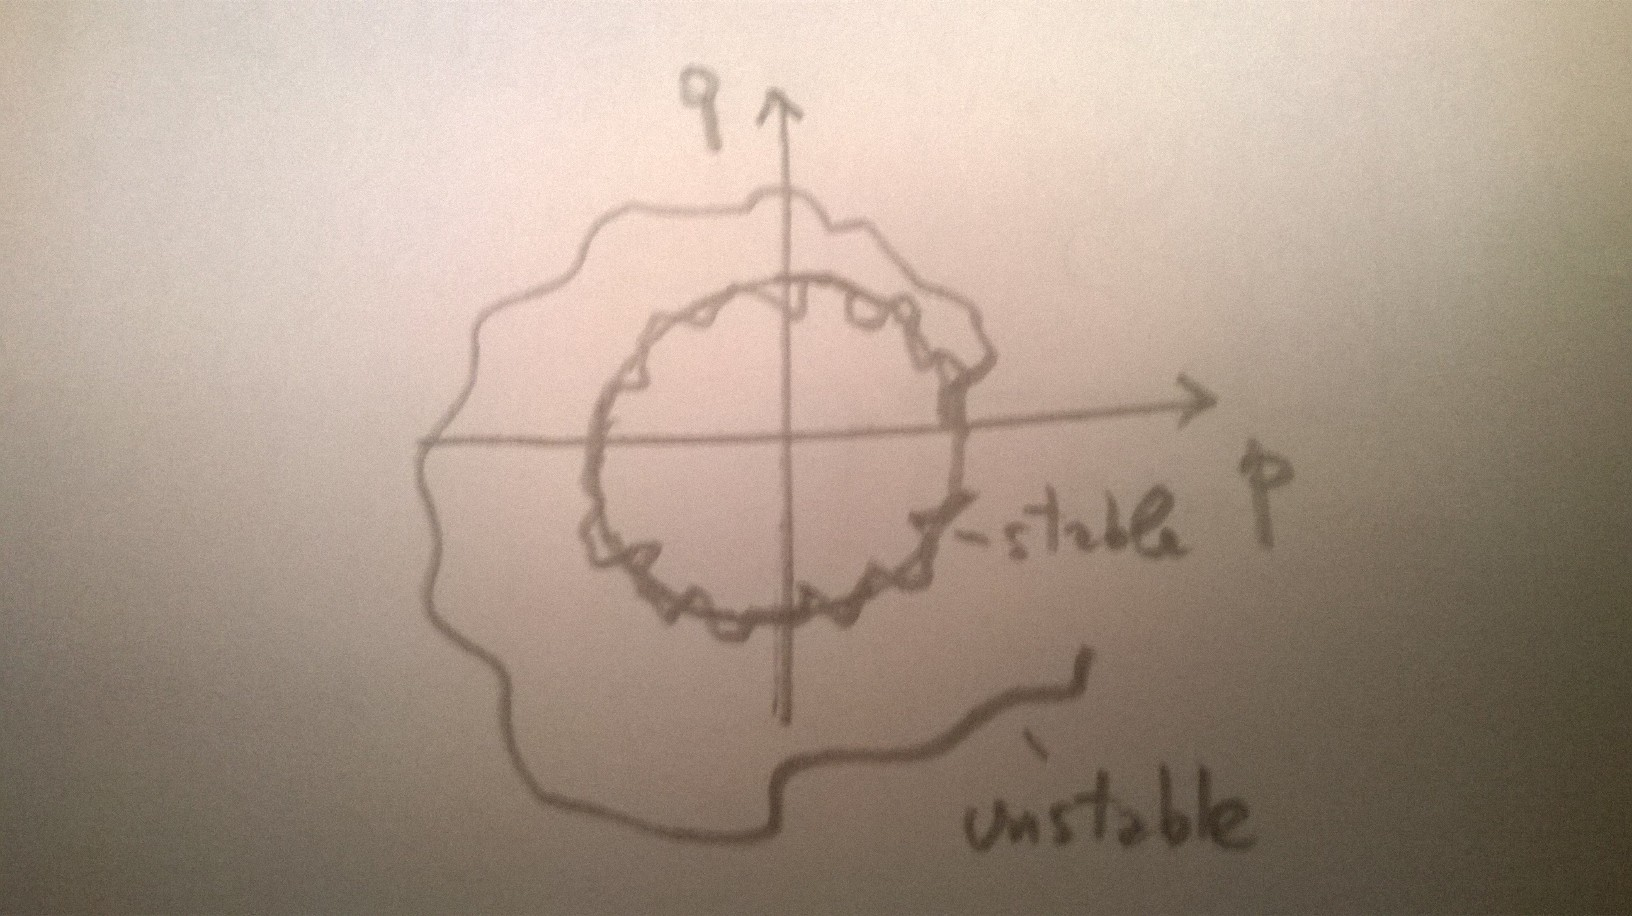
\includegraphics[width=100mm]{pic4.jpg}
\end{figure}

If we draw $H \mbox{vs} T$:

\begin{figure}[H]
\centering
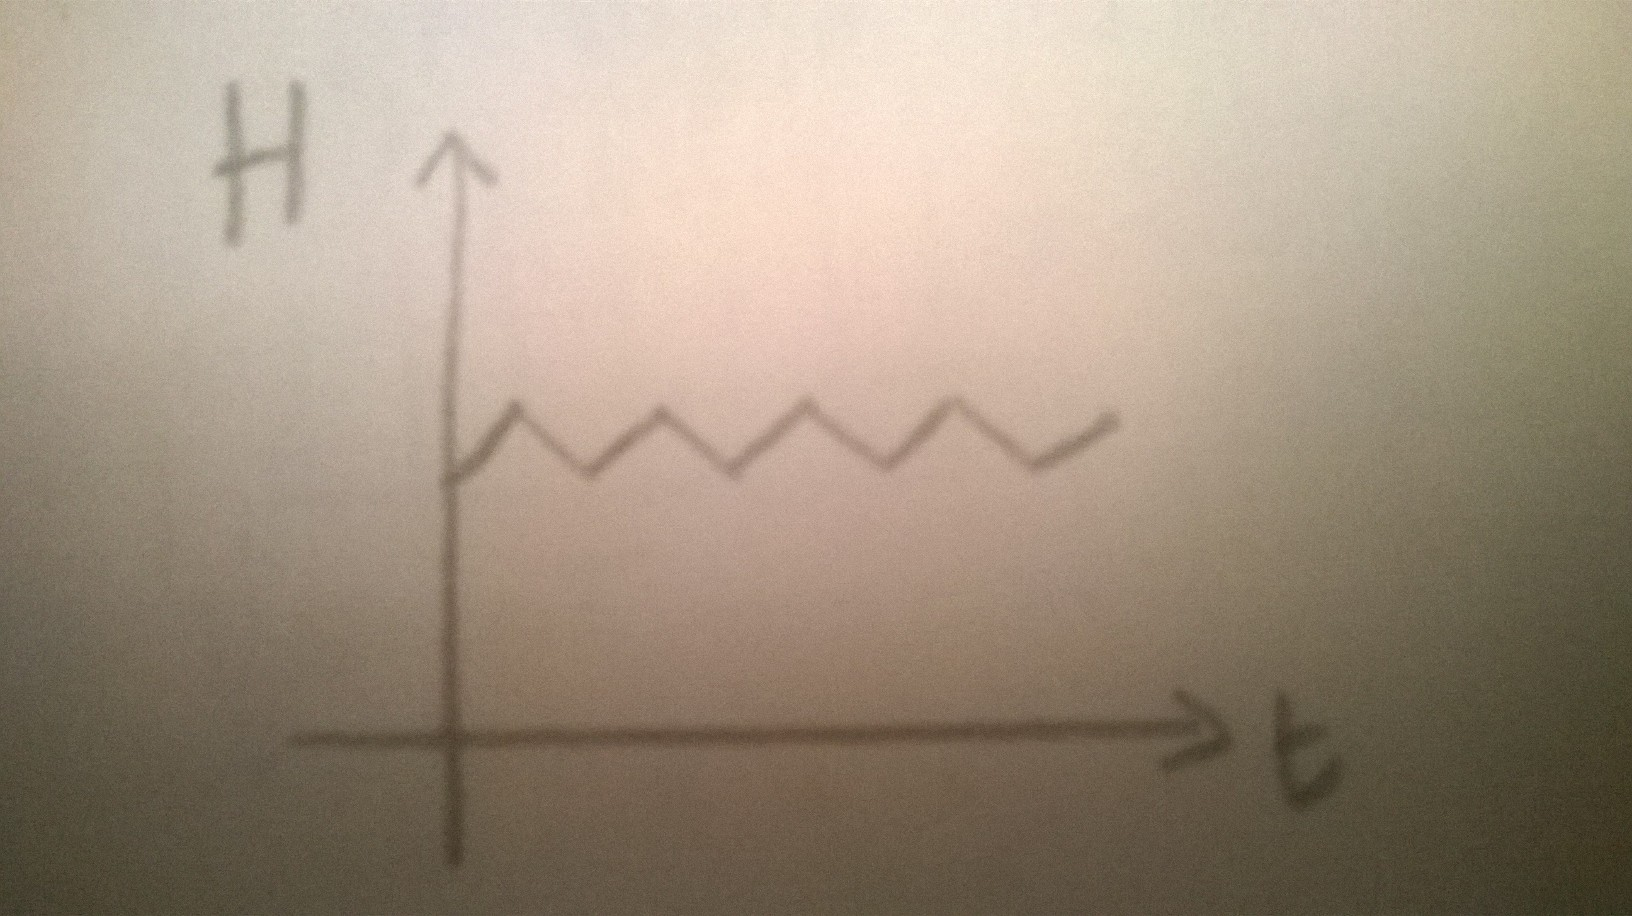
\includegraphics[width=100mm]{pic5.jpg}
\end{figure}

Every step we make an error, that comes from using an approximate hamiltonian, but errors at successive steps are anticorrelated. This is in a certain way correlated to time reversibility: if energy diverges, we expect energy to increase or decrease with the same likelihood. 

So far $\Delta t$ is the only parameter to choose and we do it in a way for which the energy is conserved.\newline
If we have more than one harmonic term, we choose $\Delta t < \frac{T_{min}}{\pi}$, that is: we choose the timestep in relation to the lowest period of all. We make a choice for the worst case.\newline
If we have unharmonicity in the potential, it will introduce a drift up or down in the energy. If this is a random error, H will increase, since it's more likely that the random point of phase space will be at a higher energy than at a lower one.

\begin{figure}[H]
\centering
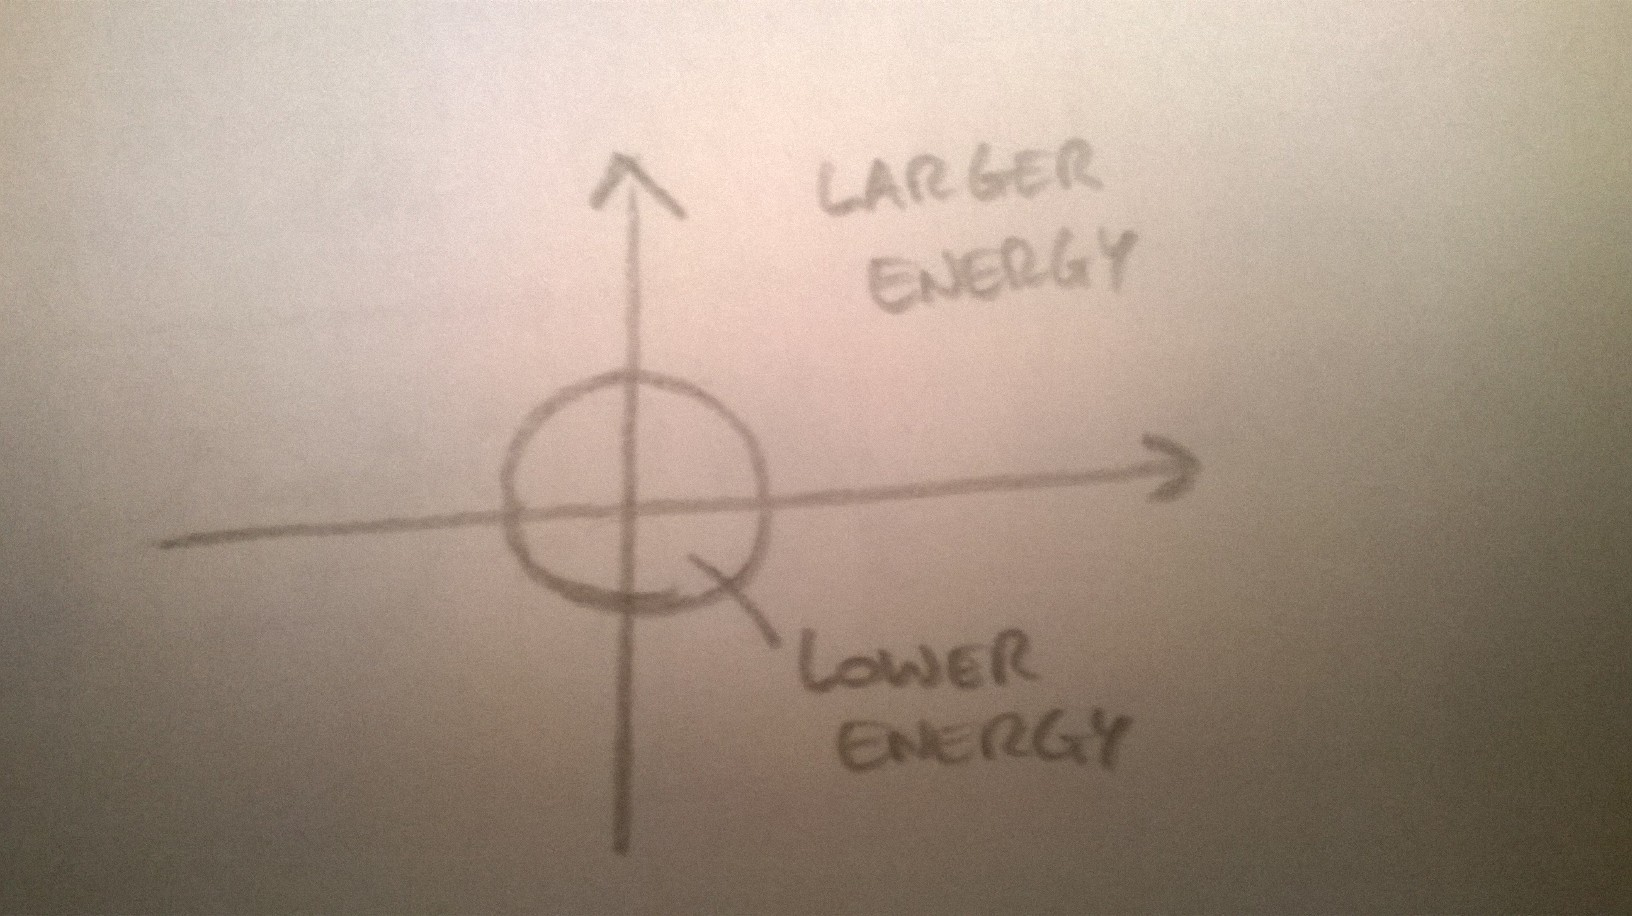
\includegraphics[width=100mm]{pic6.jpg}
\end{figure}

If the system is quasi-harmonic the drift will be very small. Decreasing $\Delta t$ makes fluctuations and slope of the drift decrease.

\begin{figure}[H]
\centering
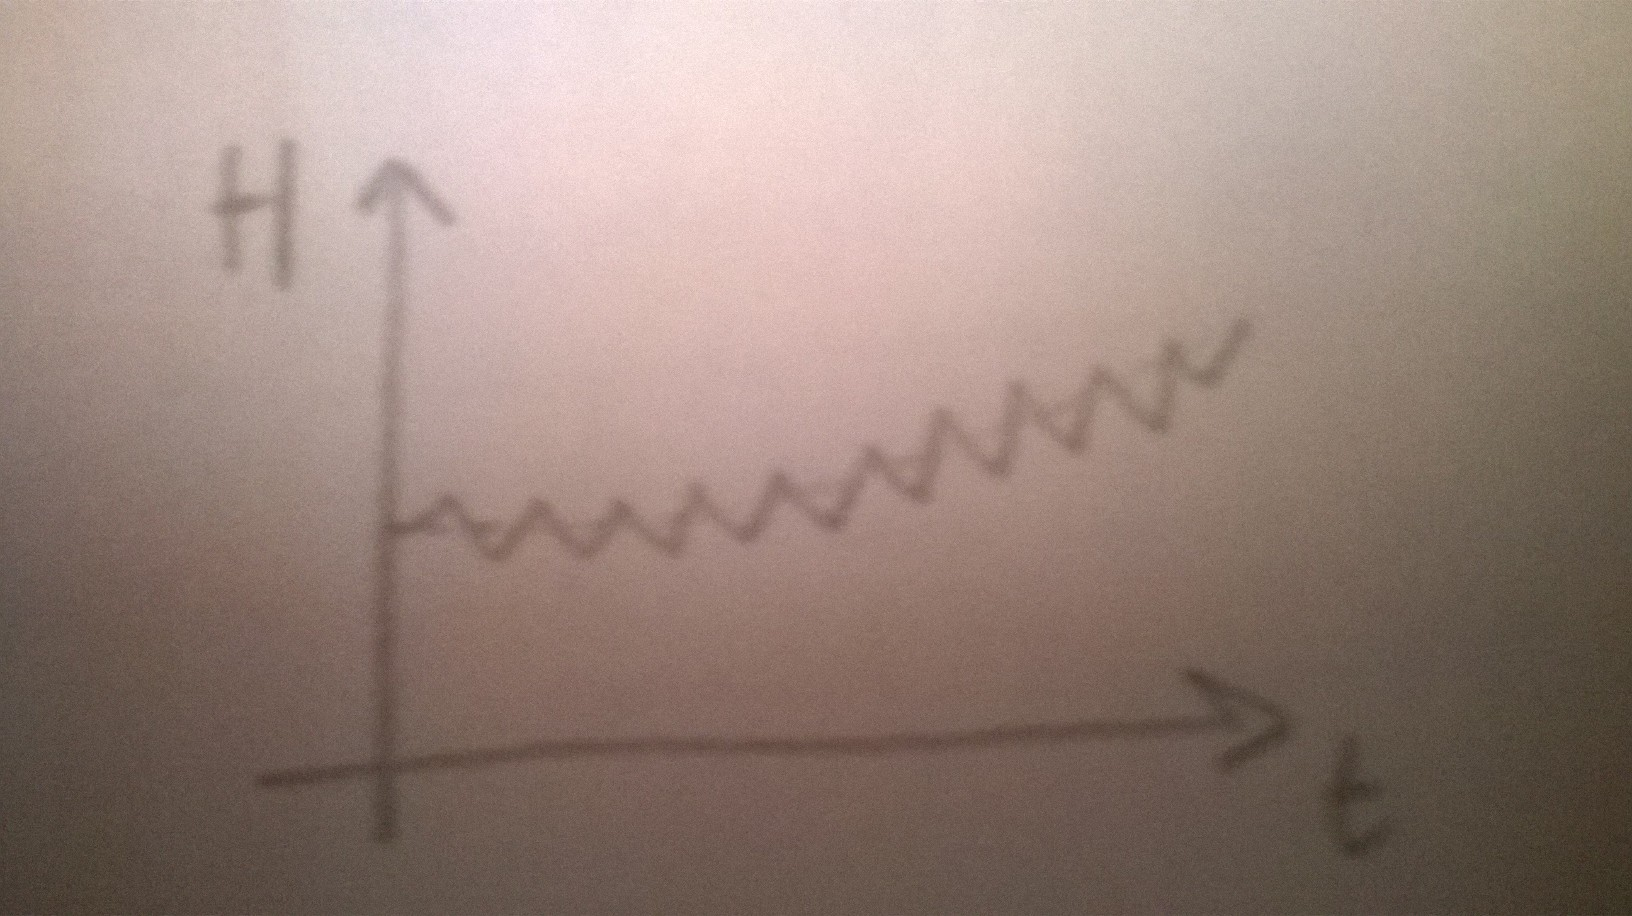
\includegraphics[width=100mm]{pic7.jpg}
\end{figure}

Usually it's said that fluctuations have to be $< k_B T$, but big systems have larger fluctuations and this is not what it's done.\newline
A useful thing is to look at drift and fluctuations to compare two simulations and say if they're equally accurate.\newline
Fluctuations scale with $\sqrt{N}$, while drift scales linearly with $N$.\newline

In molecular dynamics higher order integrators aren't used because $\epsilon \propto \Delta t^n$, so $ln \epsilon \propto N ln \Delta t$, if we plot it:

\begin{figure}[H]
\centering
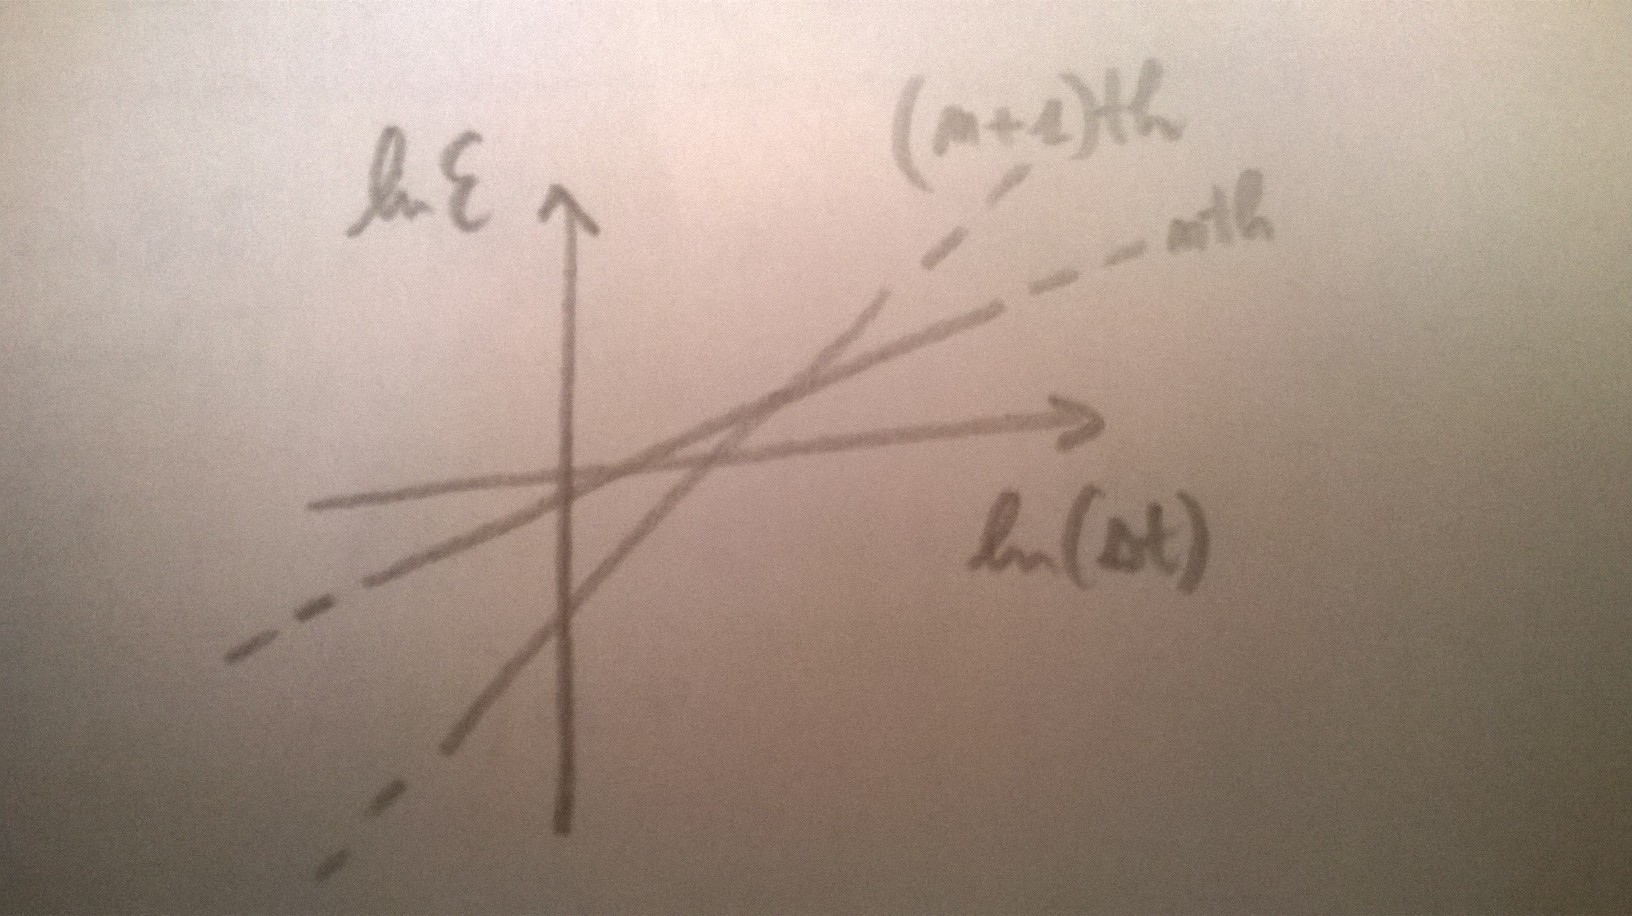
\includegraphics[width=100mm]{pic8.jpg}
\end{figure}

Higher order algorithms mean that error becomes smaller faster when decreasing $\Delta t $, but gets bigger faster when increasing timestep. Since in molecular dynamics quite large $\Delta t$ are often used, integrators of higher order are useless to this purpose, higher order algorithms are used for very short $\Delta t$ in computations like predicting trajectories of planets or artifical satellites.\newline
Another reason is that we already have approximate forces, approximate initial conditions, approximate equation... All of these introduce a much larger error than the one introduce by higher order integrators, so there's no point in using them.\newline
Often we have systems with many degrees of freedom that lead to non linear equations, in this case small differences in initial condition can lead to a very different behavior and a small mistake can become much larger.

\begin{figure}[H]
\centering
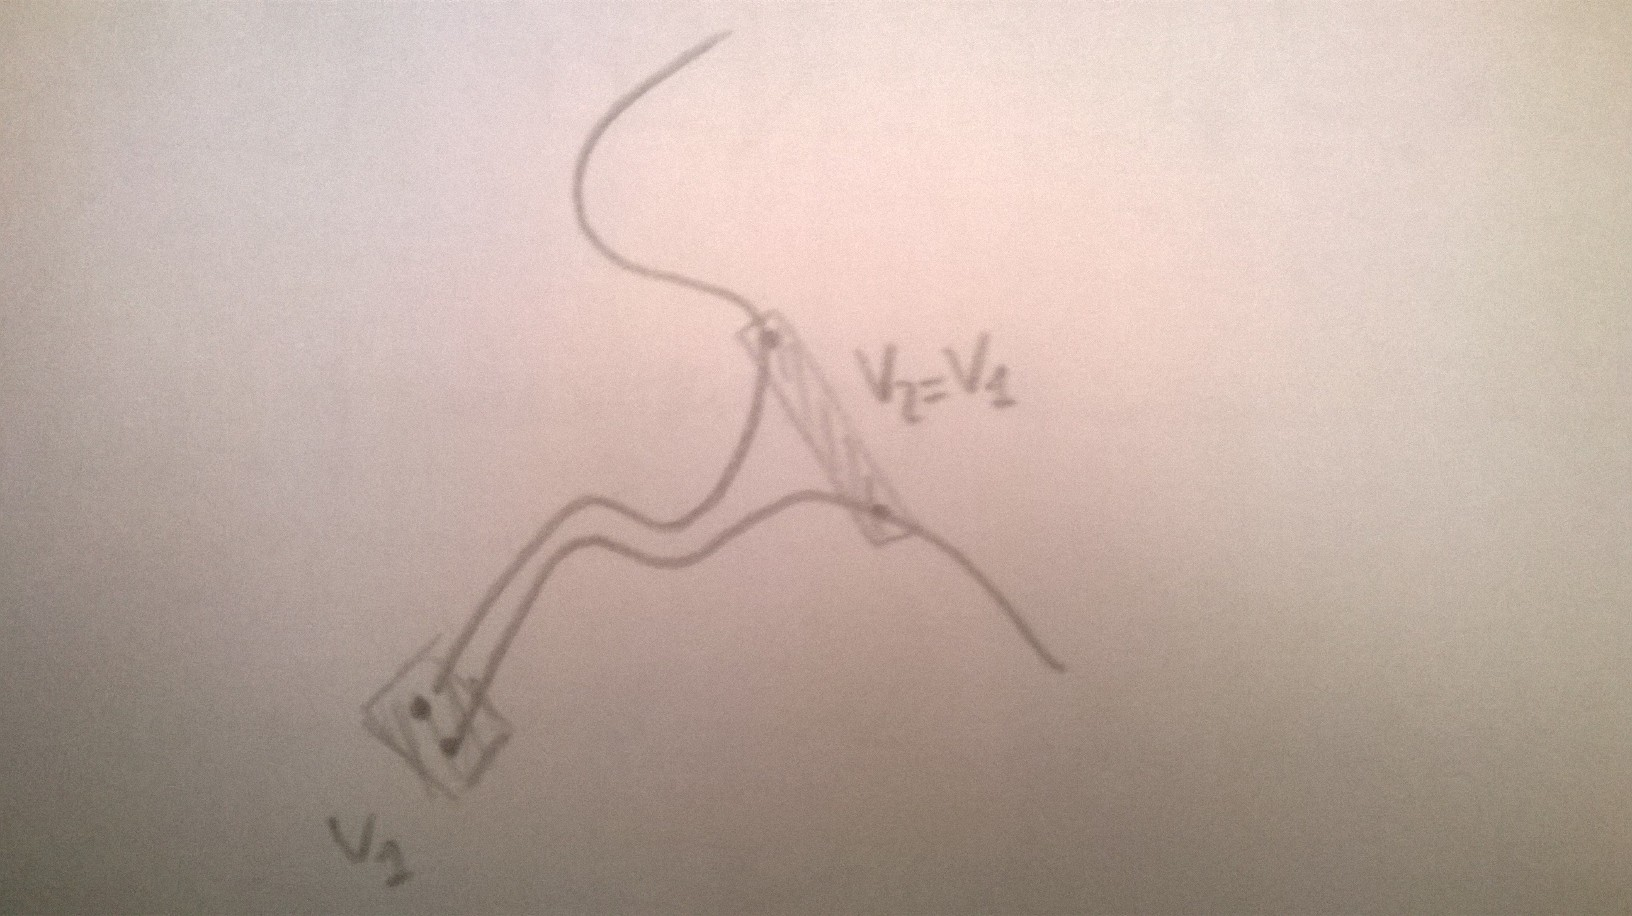
\includegraphics[width=100mm]{pic9.jpg}
\end{figure}

\section{Leap frog}

\subsection{Pseudocode}

\begin{lstlisting}
//initialize
q = ... 
p = ...

for (i = 0; i < nsteps; i++)	{
	q = q + (p/m)*deltat
	p = p + f(q)*deltat
}
\end{lstlisting}

This is the algorithm obtained by using $e^A e^B$, but with a different interpretation: $p$ at first step is $p(t+\Delta r)$ instead of $p(t)$. If we compare Velocity Verlet and Leap frog, we have:

$$q(t+\Delta t) = q(t) + \frac{p(t)}{m}\Delta t + \frac{f(t)}{2m}\Delta t^2$$

$$q(t+\Delta t) = q(t) + \frac{p(t+\frac{\Delta t}{2})}{m} \Delta t$$

where $p(t+\frac{\Delta t}{2})$ is the same velocity we get after the first update in Velocity Verlet. Actually Leap Frog is the result of combining the last operation of one step and the first of the successive step of Velocity Verlet algorithm.\newline
There isn't a big difference between the two, because they compute forces (that is the most expensive computation and actually takes about $97\%$ of the time of execution) the same number of times. In special cases where forces are relatively simple to compute and other operation weight more, Leap Frog is slightly faster. The same argument applies if we're trying to optimize at best the code: we sacrifice readability for a slightly better performance.\newline
A difference between the two algorithm is that in Velocity Verlet positions and momenta are consistent ($p(t), q(t)$), while in Leap frog they're not ($p(t+\Delta t), q(t+\frac{3}{2}\Delta t)$).

\section{Different types of ensembles and Properties of canonical ensemble}

Often it is difficult to make an experiment on a single molecule for technical reasons, and it's simpler do an experiment on an ensemble, that gives an amplified signal to measure. If we have to compre numerical simulations and experiment what we do is actually comparing an average measure on an ensemble with a time average in the simulation.\newline
We have different types of ensembles, that are named by what remains constant: NVE (microcanonical), NVT (canonical), $\mu$VT (grand canonical) and then there are others like NPT, NPH or $\mu$VE. These are used according to what the experimentalist can control.

\paragraph{Properties of canonical ensemble}

$$\rho (x) = \frac{e^{-\beta H(x)}}{\mathcal{Z}} \mbox{ with } \mathcal{Z} = \int dx e^{-\beta H(x)}$$

$$<A> = \int dx P(x) A(x)$$

$$\frac{\partial <A>}{\partial T} = -\frac{1}{k_B T^2} (-<HA> - <H><A>)$$

where $<A>$ is to be considered $<A>_T$, A doesn't depend on T but the average of A does.

$$\frac{\partial <H>}{\partial T} = \frac{1}{k_B T^2} (<H^2> - <H>^2)$$

$$H = K + U$$

$$K = \sum_i \frac{|p_i|^2}{2 m_i}$$

$$<K>_T = \frac{N_f k_B T}{2} \mbox{ Nf is the number of degrees of freedom}$$

$$\frac{\partial <K>_T}{\partial T} = \frac{N_f k_B}{2}$$

$$\frac{\partial <U>}{\partial T} = \frac{1}{k_B T^2} (<HU> - <H><U>) = \frac{1}{k_B T^2}(<U^2> -<U>^2) \mbox{ fluctuation of potential energy}$$

To compute  $c_V$, you need to compute $\frac{\partial <K>}{\partial T}$ and $\frac{\partial <U>}{\partial T}$. To compute the first one, you just need to know how many atoms are there, the second one is more difficult, because it depends on position.\newline
Notice that at constant T, $K \ne \frac{k_B T}{2}$, in fact it should be equal on average: $<K> \ne \frac{k_B T}{2}$.

$$<K^2> - <K>^2 = k_B T^2 \frac{\partial <K>}{\partial T} = \frac{N_f k_B^2 T^2}{2} \mbox{ in units of $k_B T$: } \frac{N_f}{2}$$

\begin{figure}[H]
\centering
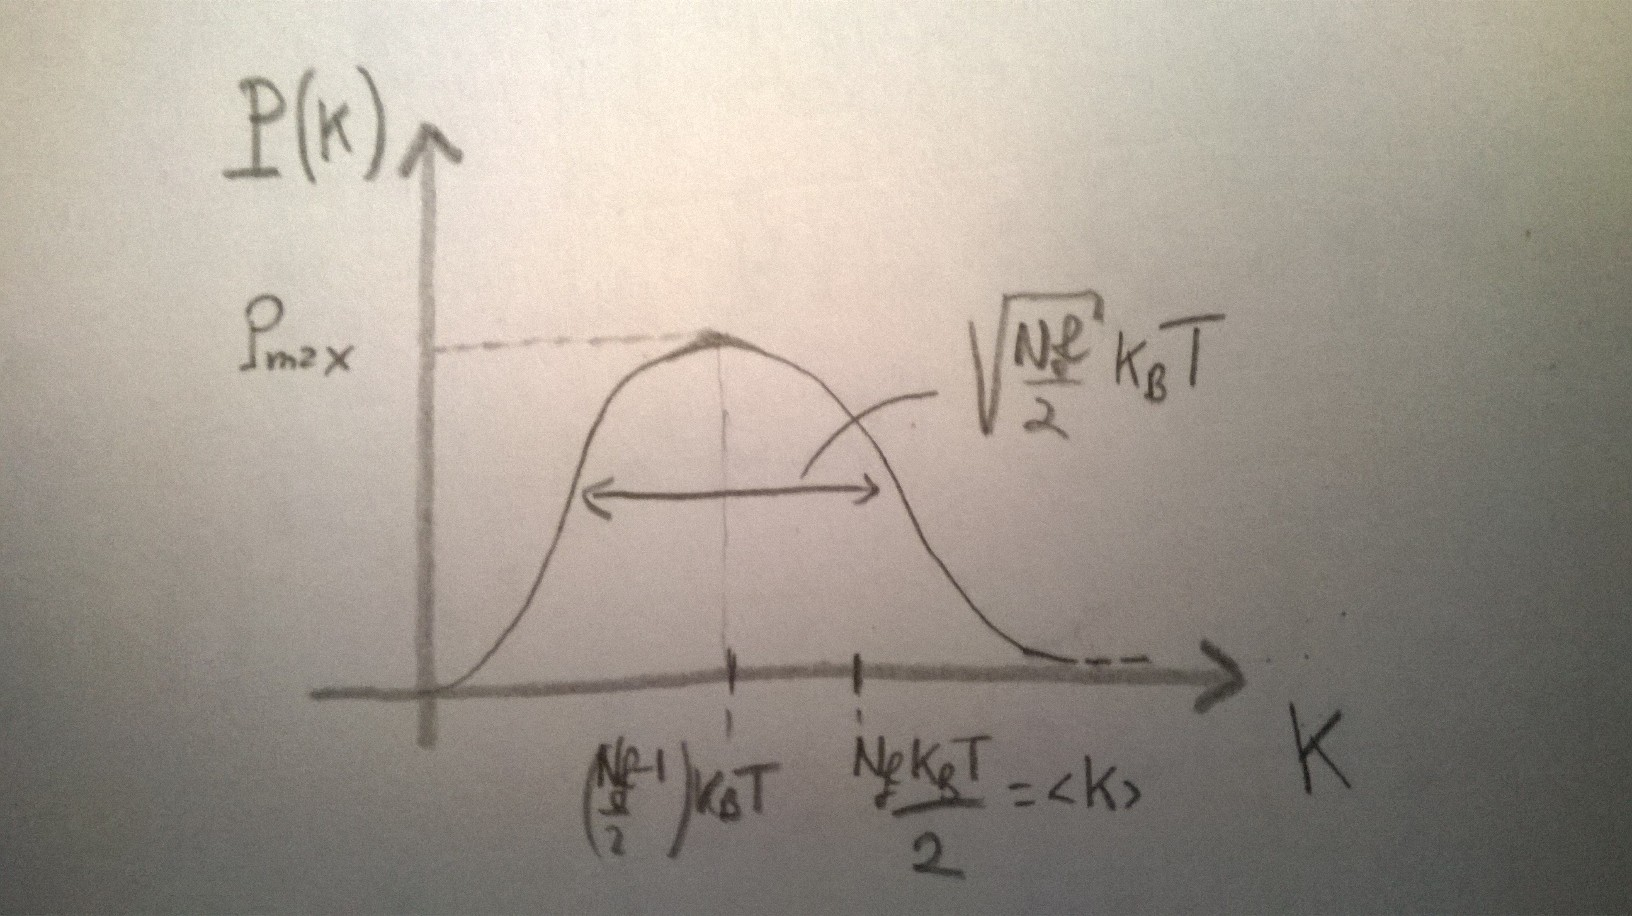
\includegraphics[width=100mm]{pic10.jpg}
\end{figure}

$$\sqrt{\frac{<K^2> - <K>^2}{<K>}} = \sqrt{\frac{2}{N_f}}$$

many degrees of freedom mean a more peaked distribution: $$<K> \propto N \mbox{, } \sigma(K) \propto \sqrt{N}$$.

We can derive the function $\mathcal{P}(K)$:

$$\mathcal{P}(K) \propto \int dp \delta(\sum_i \frac{p_i^2}{2 m_i}) e^{-\beta \sum_i \frac{p_i^2}{2m_i}} \propto e^{-\beta K} \Omega(K)$$

where $e^{-\beta K}$ says that large values of kinetic energy are not likely and $\Omega(K)$ how much the number of states changes with K.

\begin{figure}[H]
\centering
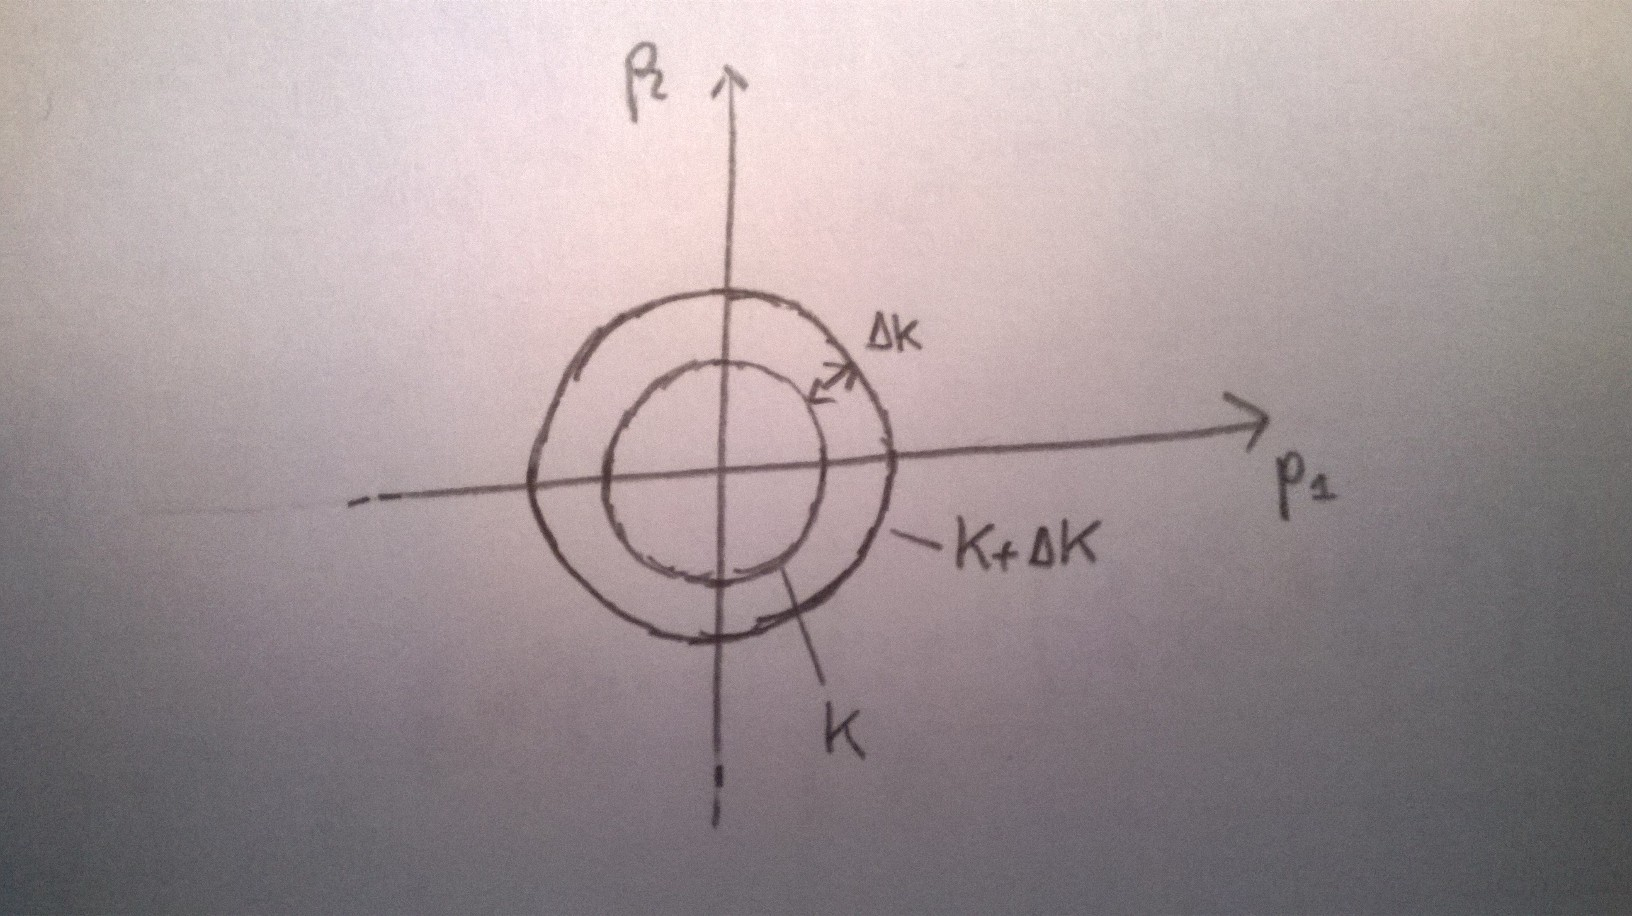
\includegraphics[width=100mm]{pic11.jpg}
\end{figure}

We want to do this in 3N dimension ($= N_f$): width of the skin (in p) per surface of inner ipersphere.

$$\Omega(K) \propto (\sqrt{K})^{N_f -1} \frac{1}{\sqrt{K}} = K^{\frac{N_f -1}{2} - \frac{1}{2}} = K^{\frac{N_f}{2}-1}$$

where $\sqrt{K}$ is the radius and $\sqrt{1/K}$ is the width of the skin, since:

$$\frac{\partial K}{\partial p} \Delta |p| = \Delta K \rightarrow \Delta K \propto \Delta|p| \rightarrow \Delta p \propto \frac{\Delta K}{K} \propto \frac{\Delta K}{\sqrt{K}}$$

so

$$\mathcal{P}(K) \propto K^{\frac{N_f}{2}-1}e^{-\beta K}$$

\begin{figure}[H]
\centering
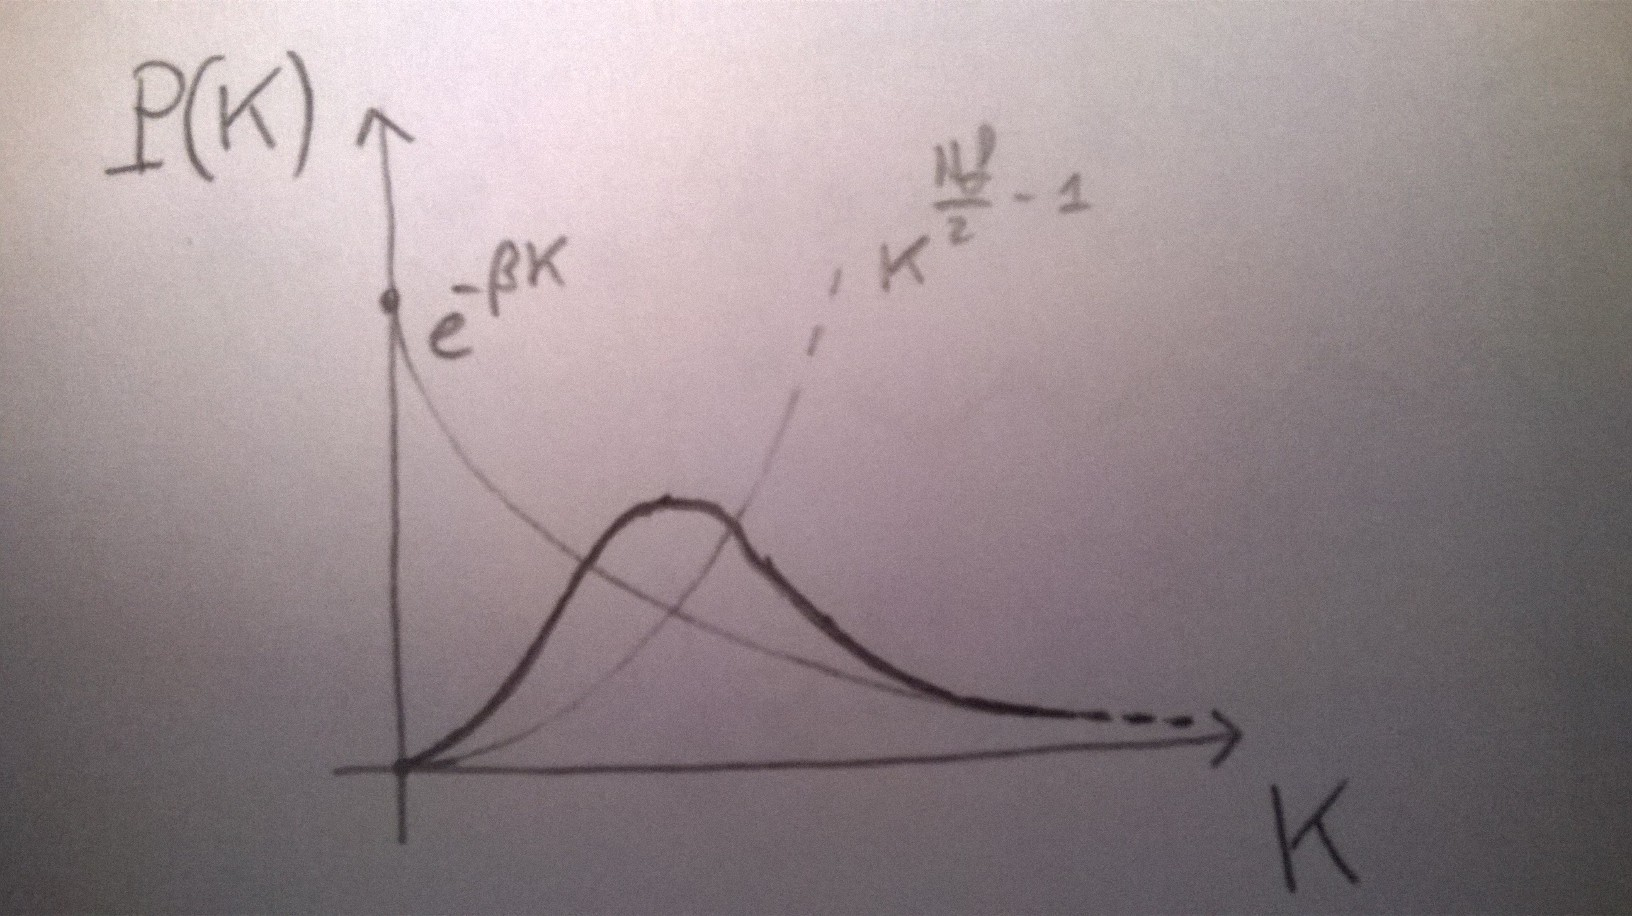
\includegraphics[width=100mm]{pic12.jpg}
\end{figure}

Doing the first derivative of $\mathcal{P}(K)$ and imposing it's equal to zero, we can find K that maximizes $\mathcal{P}$, that is $K = \left ( \frac{N_f}{2}-1 \right )k_B T$.\newline
This analysis is valid only for K, but irrespectively of the system, given that it's canonical. This holds also for U for the harmonic oscillator, because U has the same functional form of K in that case. So, \textbf{for the harmonic oscillator}:

$$\mathcal{P}(U) \propto U^{\frac{N_f}{2}-1}e^{-\beta U}$$
$$\mathcal{P}(H) \propto K^{N_f-1}e^{-\beta H} \mbox{ since degrees of freedom are 6N}$$

\section{Monte Carlo Integration Method}

Monte Carlo integration is a technique for numerical integration using random numbers. It is a particular Monte Carlo method that numerically computes a definite integral. While other algorithms usually evaluate the integrand at a regular grid, Monte Carlo randomly choose points at which the integrand is evaluated. This method is particularly useful for higher-dimensional integrals. Monte Carlo is useful also when the number of points that are contributing to the integral is a tiny fraction.\newline
Crude Monte Carlo sampling is not efficient if most of the points won't be relevant: most of the calculations will be useless.

\subsection{Markov Chain Monte Carlo}

This is a method that builds a list of points such that satisfies a prescribed distribution, even if it has a very difficult analytical form. A \textbf{Markov chain} is a random process that undergoes transitions from one state to another on a state space. It must possess a property that is usually characterized as \textit{memorylessness}: \textbf{the probability distribution of the next state depends only on the current state and not on the sequence of events that preceded it}.

\begin{itemize}
\item Choose an arbitrary point $x_0$ to be the first sample
\item propose a move
\item check if it satisfies some rule: if yes, evaluate the function, otherwise, propose a new move.
\end{itemize}

Rules to be satisfied:

\begin{itemize}
\item \textbf{reversibility}: $P(A \rightarrow B) = P(B \rightarrow A)$;
\item \textbf{ergodicity}: every point of the space can be reached in a given number of steps (tricky for continuous space, but you can define a neighborhood);
\item \textbf{stationarity}: $P(X_i)$ does not depend on i, equivalently $\bar{P} = \pi \bar{P}$: $\bar{P}$ is a stationary matrix associated to the transition matrix $\pi$, a right eigenvector of it, with eigenvalue 1.
\end{itemize}

Transition matrix $\pi$ is a stochastic matrix:

$$\sum_i \pi_{ij} = 1 \mbox{ probability of going from j to i}$$

$$\pi_{ij} \ge 0 \mbox{ equality means transition is forbidden, it can happen}$$

$$P_i^{NEW} = P_i^{OLD} + \sum_{j \ne i} \pi_{ij}P_j - \sum_{j \ne i} \pi_{ji}P_i = P_i^{OLD} + \sum_j \pi_{ij}P_j - \sum_j \pi_{ji} P_i^{OLD}$$

since $\sum_j \pi_{ji} = 1$:

$$P_i^{NEW} = \sum_j \pi_{ij}P_j$$

Another way of stating the same condition:

$$\sum_j \pi_{ij} \bar{P_j} = \sum_i \pi_{ji} \bar{P_i}$$

that means that the probability of going from i to j and from j to i is the same, so P is stationary. This condition is called \textbf{balance}.\newline
One can have a more strict condition:

$$\sum_{j\ne i} \left ( \pi_{ij}\bar{P_j} - \pi_{ji}\bar{P_i} \right ) = 0$$

so:

$$\pi_{ij}\bar{P_j} = \pi_{ji}\bar{P_i}$$

that is called \textbf{detailed balance} or also microreversibility. Detailed balance implies balance: it's a sufficient but not necessary condition. In this case every single transition is compensated by an opposite transition.\newline
Hamilton equations satisfy properties very close to detailed balance. There are notable exceptions, such as non equilibrium systems, in which this is not true: if a system is out of equilibrium, it satisfies only balance property. By the way detailed balance is not necessary in order to implement Monte Carlo algorithm, is just a way to do it.\newline
An interesting thing we find from detailed balance is:

$$\frac{\pi_{ij}}{\pi_{ji}} = \frac{\bar{P_i}}{\bar{P_j}}$$

The ratio between one move and the inverse should be equal to the ratio of P of two end states. Actually you need only to know this rate to implement a correct algorithm.

\paragraph{Examples: two and three states systems}

\begin{itemize}
\item \textbf{two state system}:

$$\bar{P_1} = x, \bar{P_2} = y$$

we have

$$\left ( \begin{array}{cc} a & b \\ c & d \end{array} \right ) \left ( \begin{array}{c} x\\ y \end{array} \right ) = \left ( \begin{array}{c} x\\ y \end{array} \right )$$

since $\pi$ must be a stochastic matrix:

$$\left ( \begin{array}{cc} 1-c & b \\ c & 1-b \end{array} \right ) \left ( \begin{array}{c} x\\ y \end{array} \right ) = \left ( \begin{array}{c} x\\ y \end{array} \right )$$

that gives $cx = by$, that is: $\frac{c}{b}=\frac{y}{x}$

\begin{figure}[H]
\centering
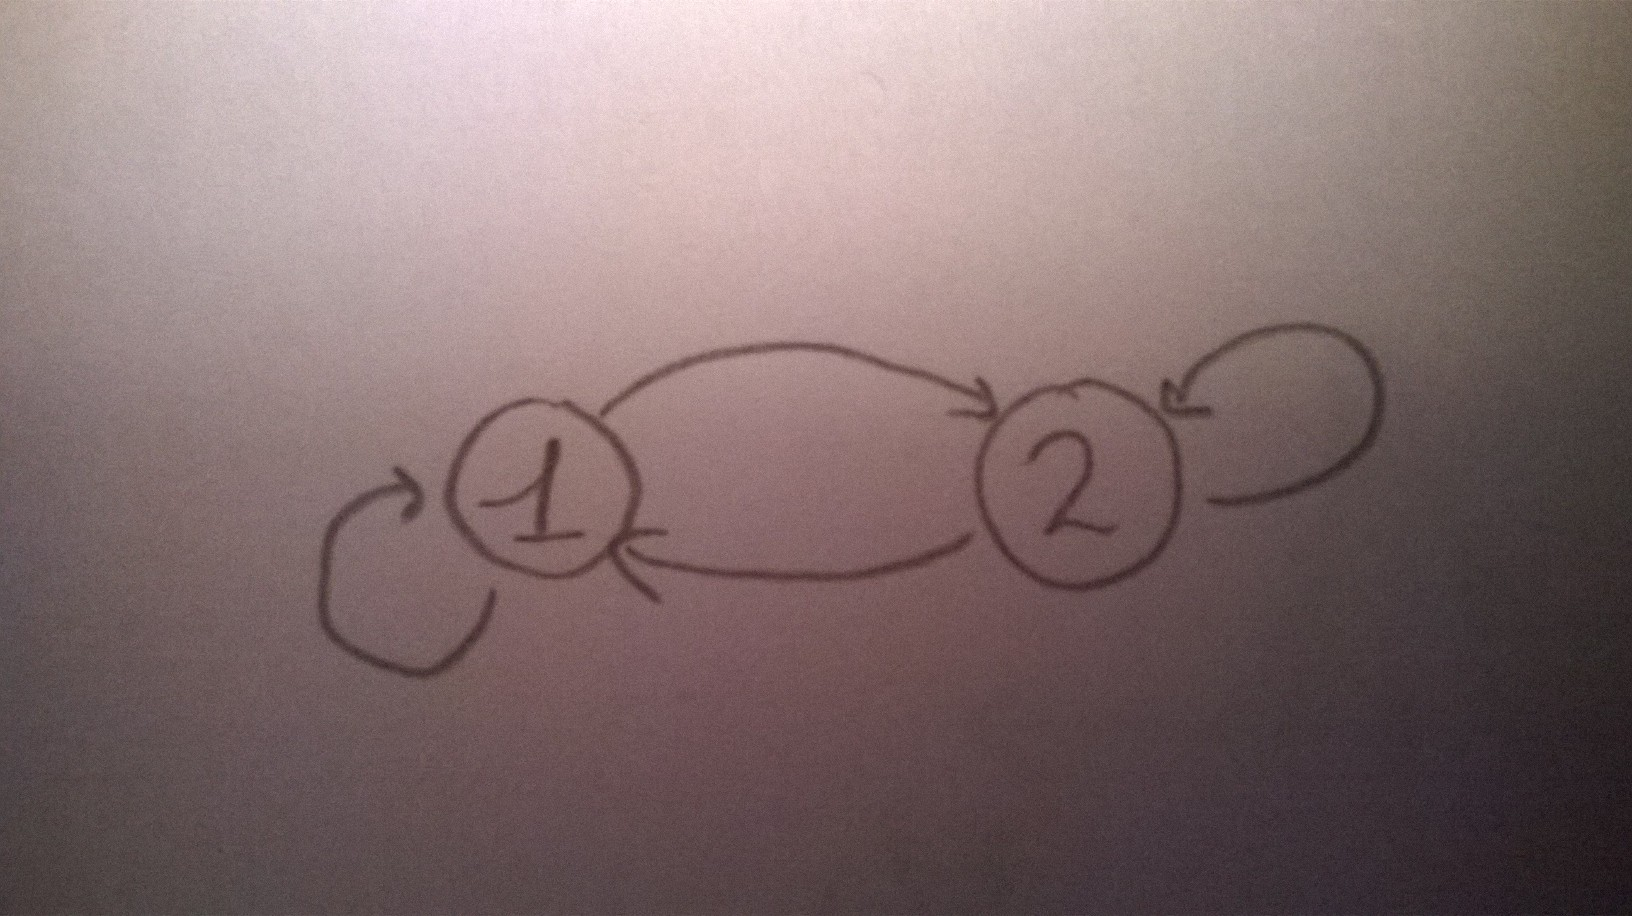
\includegraphics[width=100mm]{pic13.jpg}
\end{figure}

All arrows entering compensate with arrows exiting. In this case balance implies detailed balance (actually it's the same thing, since there is no sum to do).

\item \textbf{three states stystem}:

\begin{figure}[H]
\centering
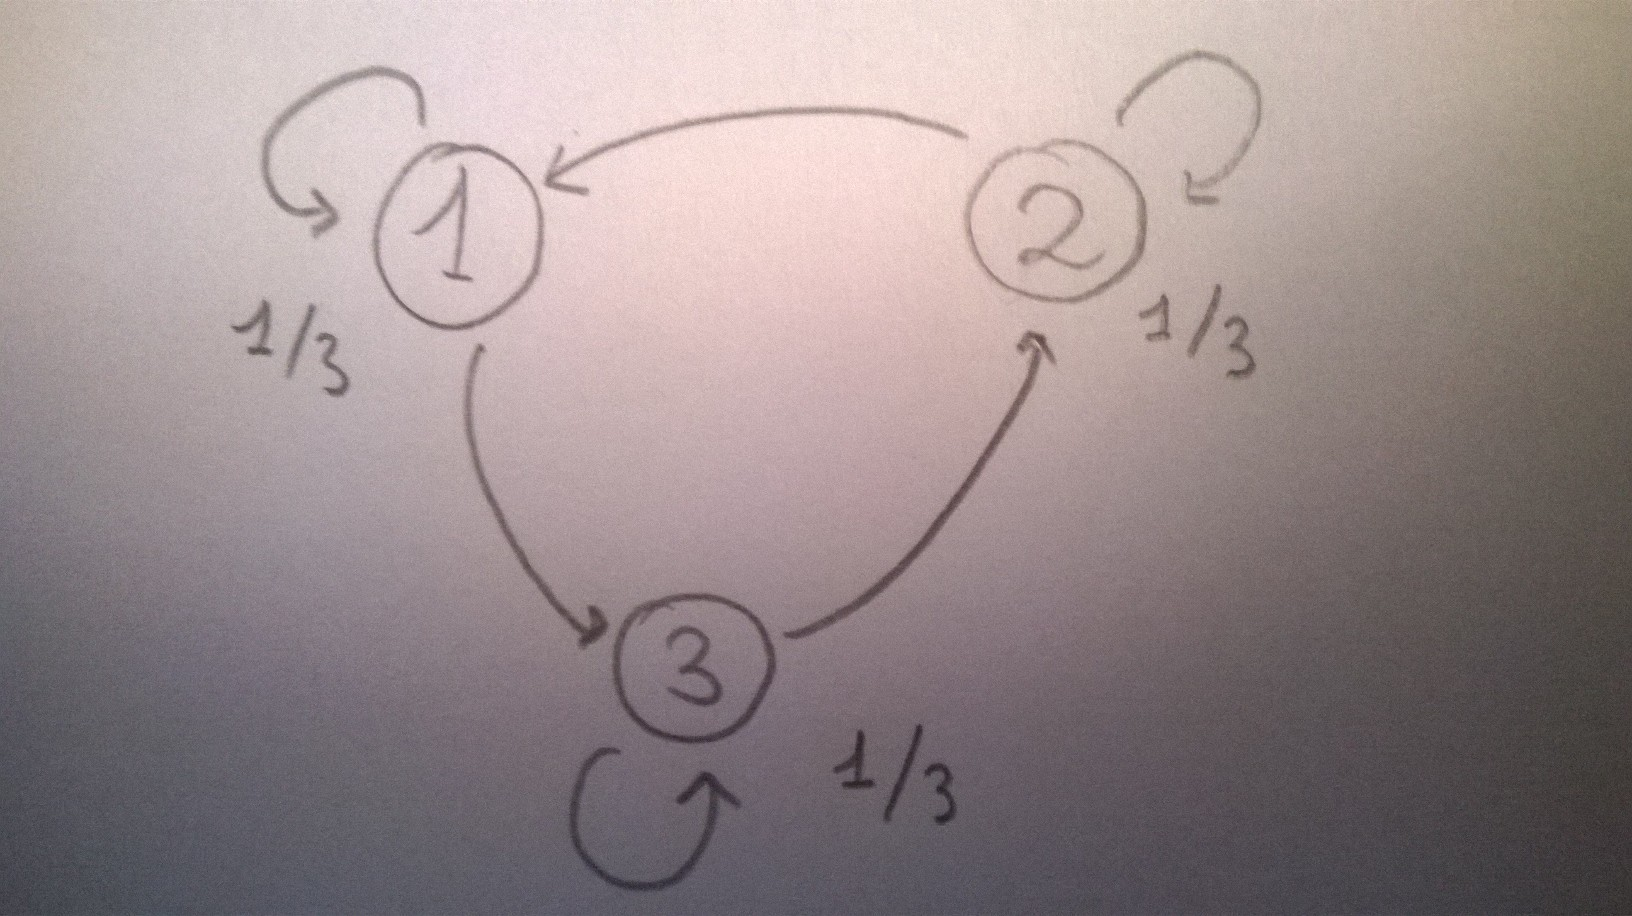
\includegraphics[width=100mm]{pic14.jpg}
\end{figure}

In this case detailed balance isn't satisfied, but balance is.There is a net current different from zero.

\begin{figure}[H]
\centering
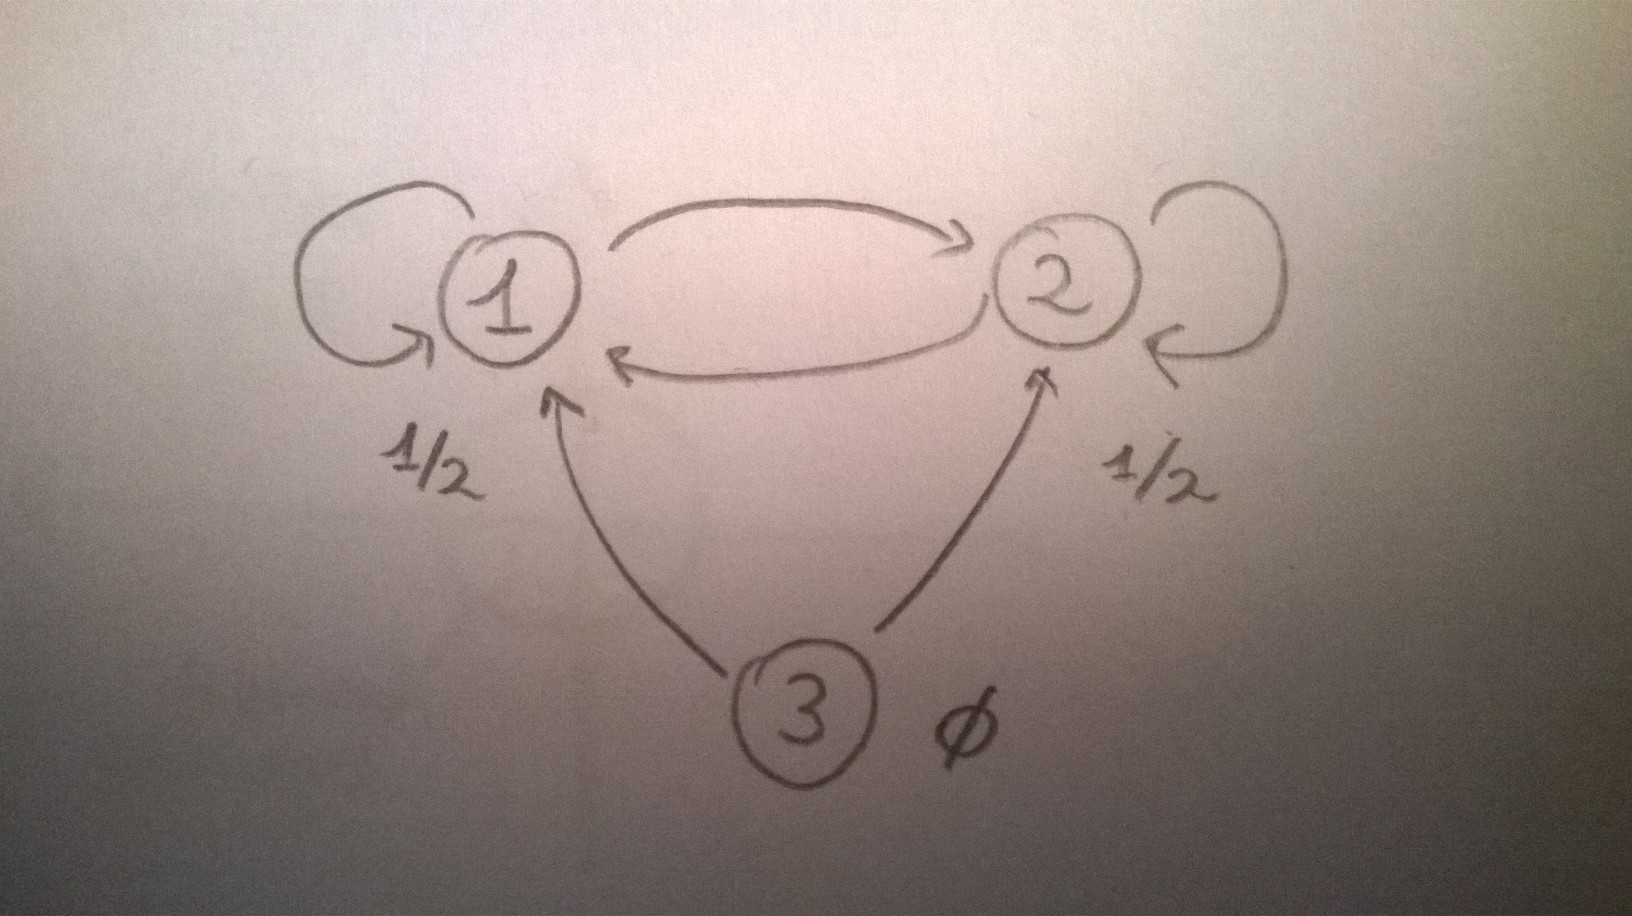
\includegraphics[width=100mm]{pic15.jpg}
\end{figure}

$$\pi = \left ( \begin{array}{ccc} 1-x & x & x \\ x & 1-x & x \\ 0 & 0 & 1-2x \end{array} \right )$$

The system in its entirety is not ergodic, but if we consider only 1 and 2 it is. Actually the ergodicity we're interested in is the condition in which the choice of initial state doesn't influence the final state of the system.

\begin{figure}[H]
\centering
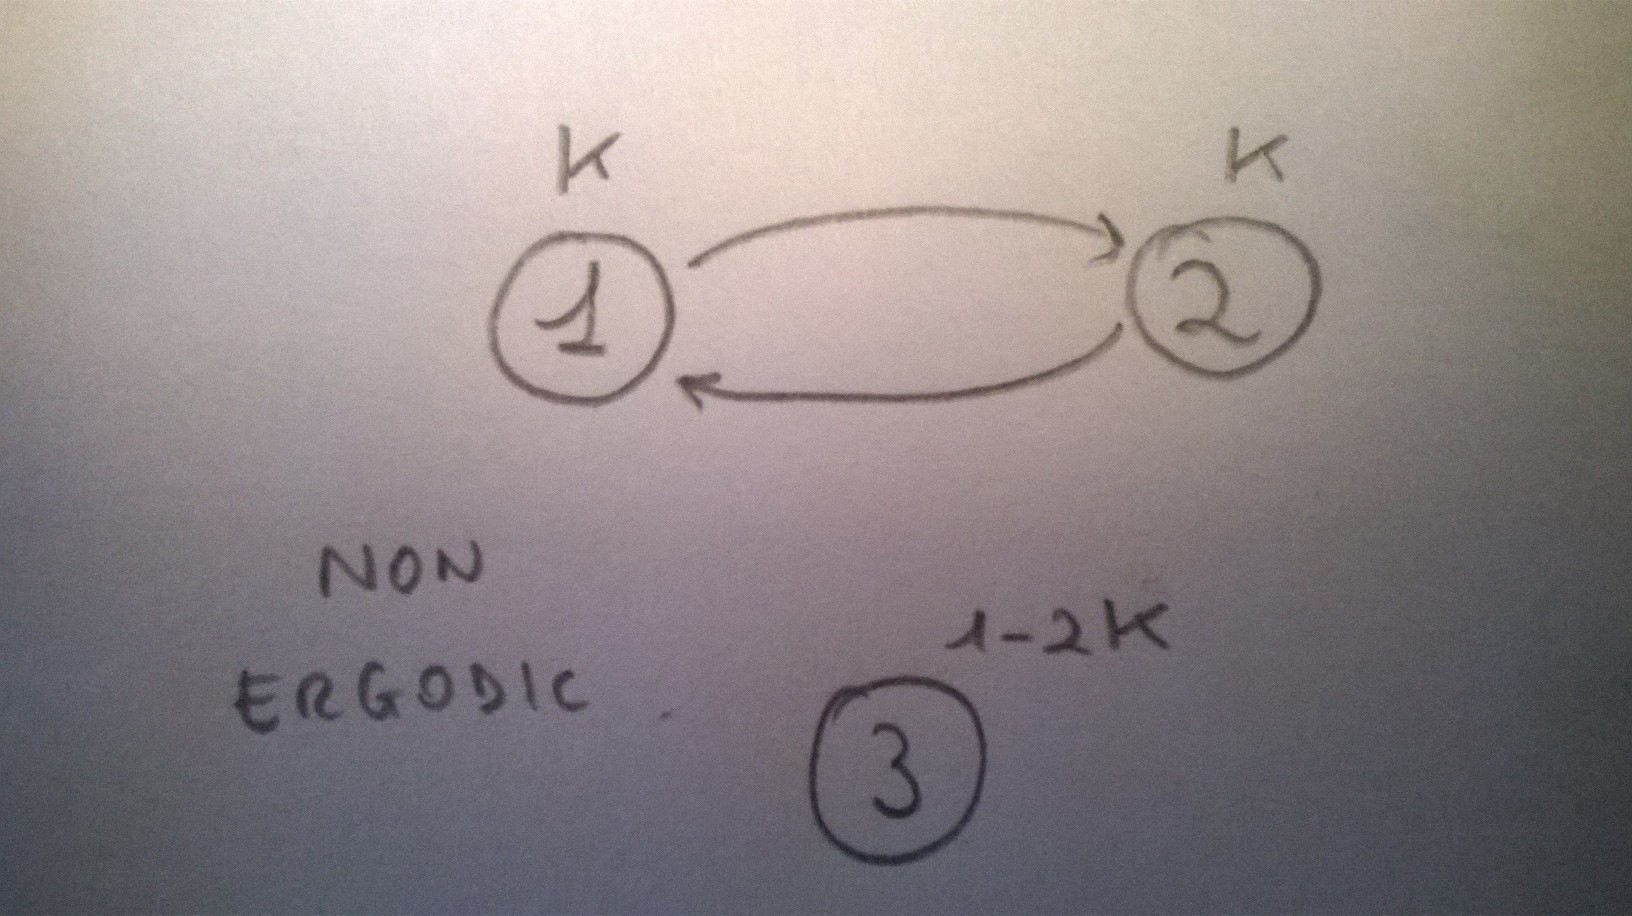
\includegraphics[width=100mm]{pic16.jpg}
\end{figure}

$$\pi = \left ( \begin{array}{ccc} 1-x & x & 0 \\ x & 1-x & 0 \\ 0 & 0 & 1 \end{array} \right )$$

This is a non-ergodic system. It's like putting together two systems that don't see each other. This is a nasty case: if I start a Monte Carlo simulation from state 3 I will have convergence, but also if I start from state 1 or 2, however the results will be different. This is a very difficult mistake to find and we have to be very careful.
\end{itemize}

Physics meaning: \textbf{detailed balance means there is no net current and describes equilibrium, while balance means there is a net current and describes non equilibrium}.

\subsection{Metropolis algorithm and Pseudocode}

\begin{figure}[H]
\centering
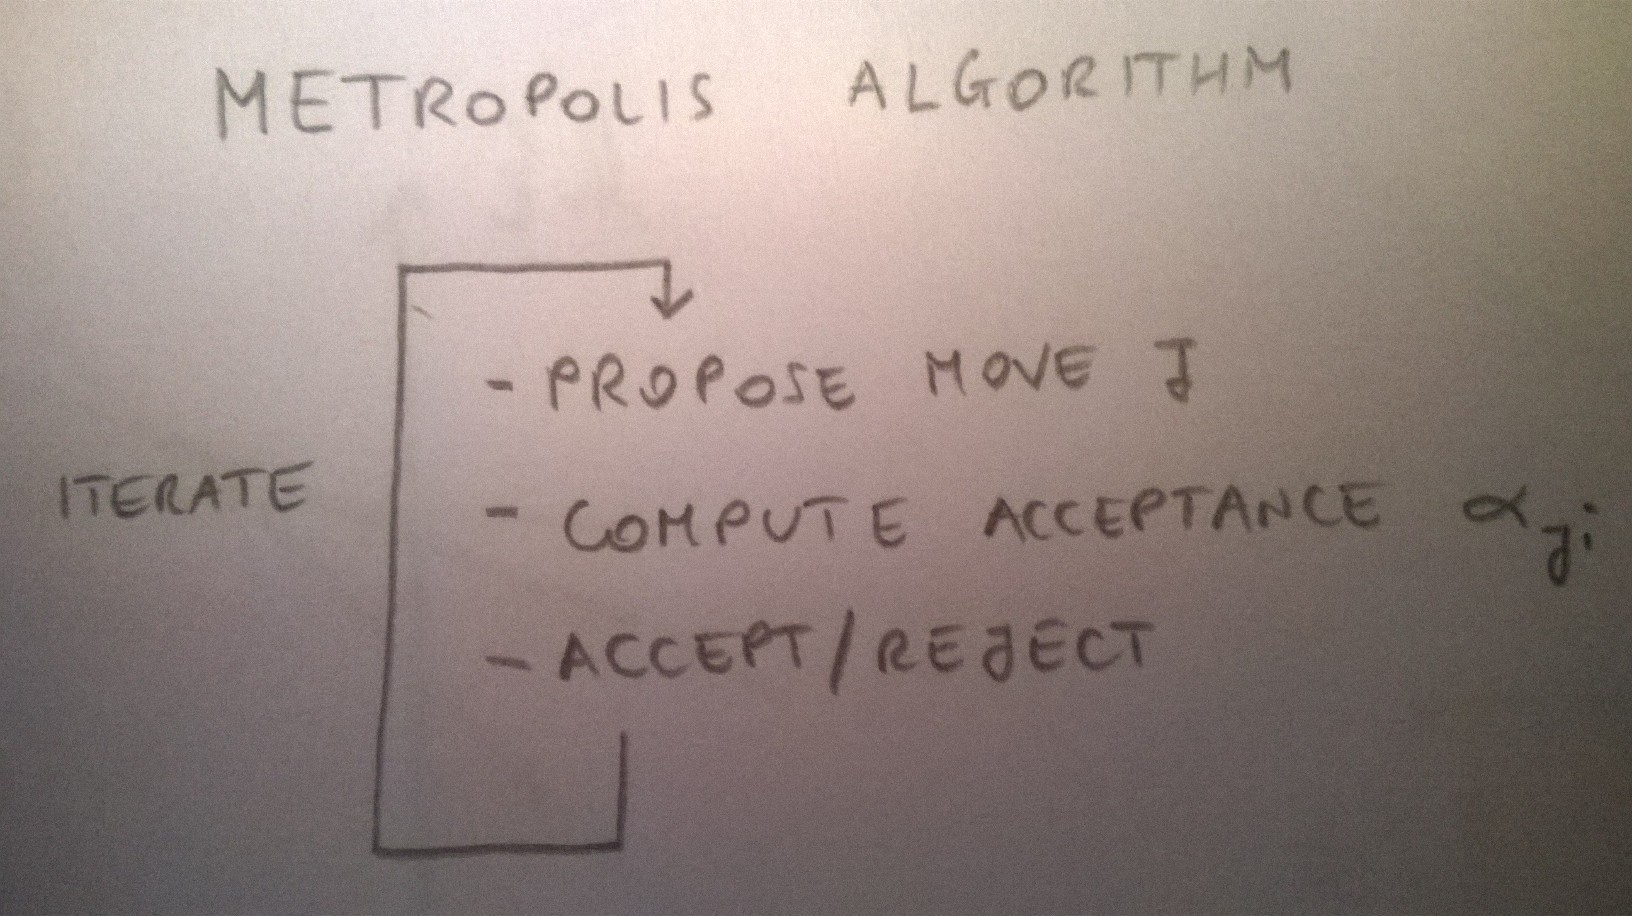
\includegraphics[width=100mm]{pic17.jpg}
\end{figure}

$$\pi_{ji} = (\mbox{probability of proposing move j})\cdot (\mbox{probability of accepting it}) = M_{ji} \cdot \alpha_{ji}$$

$$\frac{M_{ji}\alpha_{ji}}{M_{ij}\alpha_{ij}} = \frac{\bar{P_j}}{\bar{P_i}} = \mbox{ detailed balance} \rightarrow \frac{\alpha_{ji}}{\alpha{ij}} = \frac{\bar{P_j}M_{ij}}{\bar{P_i}M_{ji}} = e^{-\beta(H_j - H_i)}frac{M_{ij}}{\bar{M_ji}}$$

The choice of Metropolis is to take:

$$\alpha_{ji} = \mbox{ min}\left \{ 1, \frac{\bar{P_j}M_{ij}}{\bar{P_i}M_{ji}} \right \}$$

\paragraph{Pseudocode}

\begin{lstlisting}
//initialize
i = ... 

for (int istep = 0; istep < nsteps; istep++)	{
	
	//for integer i, j
	if(rand() > 0.5)	{
		j = i + 1
		} else	{
		j = i - 1
	}
	
	/*for real i, j
	if(rand() > 0.5)	{
		j = i + (rand() - 0.5)*delta
		} */
		
	/*not time reversible
	if(rand() > 2/3)	{
		j = i + 1
		}	else	{
		j = i - 1
		}
		
	in this case I have to compute a different alpha in each branch, since Mij and Mji are different*/
	
	alpha = exp(-beta*(h(j)-h(i)))
	
	if(alpha > rand())	{
		i = j
		}
		
	/*this condition can be refined: 
	if(alpha > 1 || ( alpha <1 && alpha > rand() )) 
	in this case i generate only the random numbers that I need and the code is optimized*/
	
	print i
	
}

/*
Notice that other choices for the move could lead to non ergodicity, for example:
Case of integers i,j: 
- j = i + 2: parity of i is conserved. Every time the system is not ergodic, there is a conserved quantity.
- case of real i, j: j = i + rand()
This can happen even if P is stationary.
*/
\end{lstlisting}

If $X_i$ were independent, for $N \to \infty$ we would made an error $\sim \frac{\sigma}{\sqrt{N}}$, where $\sigma$ is the standard deviation.\newline
We don't have independent $X_i$, each point is close to the previous one, so we have a larger error: 

$$\frac{\sigma}{\sqrt{\frac{N}{N_{correlation}}}}$$

We can implement Markov Chain Monte Carlo using a different rule: \textbf{symmetric rule}. In this case probability of acceptance is given by:

$$\alpha = \frac{\mathcal{X}}{1+\mathcal{X}} = \frac{\bar{P_j}}{\bar{P_i}+\bar{P_j}} \mbox{ where } \mathcal{X}=\frac{\bar{P_j} M_{ij}}{\bar{P_i} M_{ji}}$$

In this case we look at relative probability to make a choice. By the way Metropolis algorithm is considered the best choice, since it has the highest acceptance rate and so the least waste of calculations. If we'd try to increase $\alpha_{Metropolis}$, we'd end up with an $\alpha > 1$ for the reverse move, so this is the best we can get.\newline
Actually one should choose $\alpha$ in order to optimize the product $\alpha \cdot \Delta$, where $\Delta$ is the typical size of moves and the plot goes like this:

\begin{figure}[H]
\centering
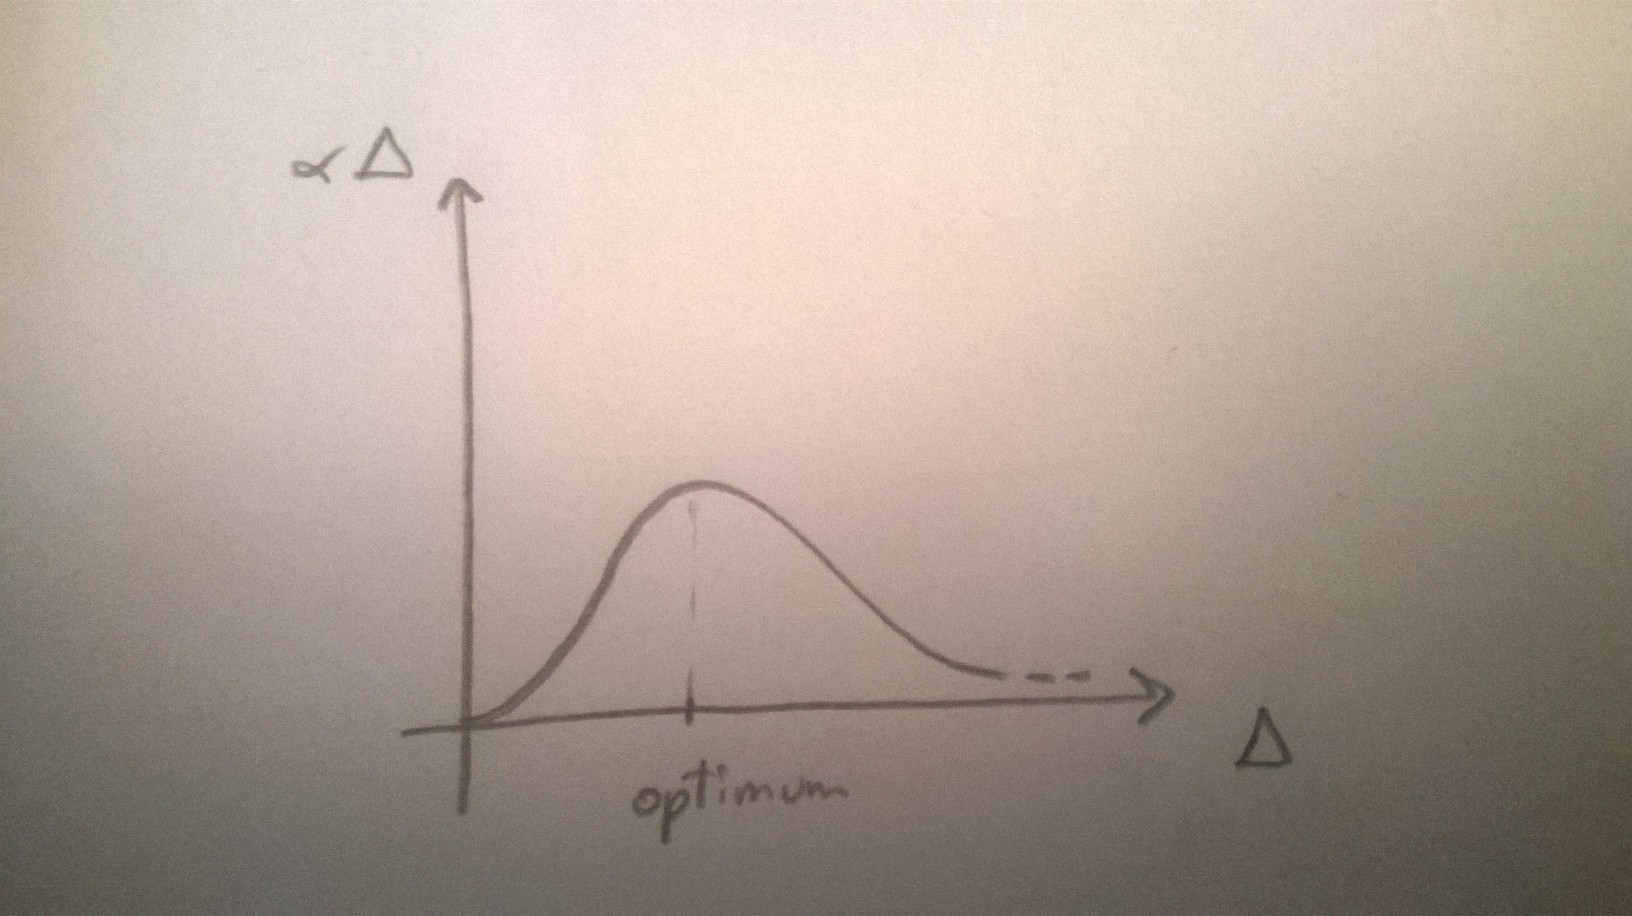
\includegraphics[width=100mm]{pic18.jpg}
\end{figure}



\end{document}